\documentclass[aspectratio=169]{beamer}
% Shared preamble for ml/ slide decks.
% Each lecture .tex starts with:
%   \documentclass[aspectratio=169]{beamer}
%   % Shared preamble for ml/ slide decks.
% Each lecture .tex starts with:
%   \documentclass[aspectratio=169]{beamer}
%   % Shared preamble for ml/ slide decks.
% Each lecture .tex starts with:
%   \documentclass[aspectratio=169]{beamer}
%   \input{../preamble}
% Compile from inside the chapter folder so \input{../preamble} resolves.

\usetheme{default}
\usecolortheme{dove}

\setbeamertemplate{navigation symbols}{}
\setbeamertemplate{footline}{%
  \hfill{\large\insertframenumber\,/\,\inserttotalframenumber}\hspace{0.8em}\vspace{0.5em}%
}

% Project palette (existing, kept for backwards compatibility with deferred/*)
\definecolor{popblue}{RGB}{52, 101, 164}
\definecolor{sampred}{RGB}{204, 0, 0}
\definecolor{paramgreen}{RGB}{0, 140, 70}
\definecolor{warnred}{RGB}{180, 40, 40}
\definecolor{orange1}{RGB}{220, 120, 0}
\definecolor{violet1}{RGB}{120, 50, 160}
\definecolor{lightbg}{RGB}{245, 245, 250}

% Armenian flag palette (use these for any 3-color highlight; per CLAUDE.md).
% "Nice versions": slightly de-saturated from the official spec for slide use,
% so they don't burn out under projector colors. Originals kept as *_pure.
\definecolor{armred}{RGB}{200, 30, 40}      % nice red (official #D90012 muted)
\definecolor{armblue}{RGB}{30, 70, 160}     % nice blue (official #0033A0 muted)
\definecolor{armorange}{RGB}{230, 160, 30}  % nice orange (official #F2A800 muted)
\definecolor{armred_pure}{HTML}{D90012}     % official Armenian flag red
\definecolor{armblue_pure}{HTML}{0033A0}    % official Armenian flag blue
\definecolor{armorange_pure}{HTML}{F2A800}  % official Armenian flag orange

\setbeamercolor{frametitle}{fg=popblue}
\setbeamercolor{title}{fg=popblue}

\usepackage{pgfplots}
\usepackage{tikz}
\usetikzlibrary{shapes, arrows.meta, positioning, calc, decorations.pathreplacing, patterns, matrix}
\pgfplotsset{compat=1.18}
\usepackage{amsmath, amssymb, amsfonts}
\usepackage{bm}
\usepackage{dsfont}
\usepackage{array}
\usepackage{pifont}
\usepackage{colortbl}
\usepackage{fontenc}

% Callout boxes. Purely additive - existing decks are unaffected.
% Usage: \begin{tcolorbox}[colback=armblue!8, colframe=armblue, boxrule=0.6pt, arc=2pt,
%                          title=\textbf{Key idea}] ... \end{tcolorbox}
% Palette convention (ml/SLIDE_STYLE.md): armblue=key idea, armred=trap/warning,
% paramgreen=takeaway or "Next", armorange=watch-out.
\usepackage[most]{tcolorbox}

% Cleaner table rules (\toprule, \midrule, \bottomrule). Also purely additive.
\usepackage{booktabs}

% \cancel{...} for struck-through terms in derivations (added 2026-08-11 for the
% importance-sampling frame in ch11_rl, where the dynamics cancel). Purely additive.
\usepackage{cancel}

% Minimal ML notation macros (subset of slds-lmu latex-math/basic-ml.tex).
% Kept here so we don't have to inline-expand every \thetav, \xv, etc.
% when porting upstream slides.
\newcommand{\R}{\mathds{R}}
\newcommand{\N}{\mathds{N}}
\newcommand{\E}{\mathds{E}}
\newcommand{\Xspace}{\mathcal{X}}
\newcommand{\Yspace}{\mathcal{Y}}
\newcommand{\Hspace}{\mathcal{H}}
\newcommand{\D}{\mathcal{D}}
\newcommand{\Dtrain}{\mathcal{D}_{\text{train}}}
\newcommand{\Dtest}{\mathcal{D}_{\text{test}}}
\newcommand{\xv}{\mathbf{x}}
\newcommand{\yv}{\mathbf{y}}
\newcommand{\Xmat}{\mathbf{X}}
\newcommand{\id}{\mathbf{I}}
\newcommand{\thetav}{\bm{\theta}}
\newcommand{\thetah}{\hat{\bm{\theta}}}
\newcommand{\lamv}{\bm{\lambda}}
\newcommand{\fx}{f(\xv)}
\newcommand{\fxt}{f(\xv \,|\, \bm{\theta})}
\newcommand{\fxi}{f\!\left(\xv^{(i)}\right)}
\newcommand{\fh}{\hat{f}}
\newcommand{\fxh}{\hat{f}(\xv)}
\newcommand{\yh}{\hat{y}}
\newcommand{\yih}{\hat{y}^{(i)}}
% \xi clashes with the Greek letter \xi; write \xv^{(i)} inline instead.
\newcommand{\yi}[1][i]{y^{(#1)}}
\newcommand{\xyi}[1][i]{\left(\xv^{(#1)},\, y^{(#1)}\right)}
\newcommand{\thx}{\bm{\theta}^\top \xv}
\newcommand{\sumin}{\sum_{i=1}^{n}}
\newcommand{\sumjp}{\sum_{j=1}^{p}}
\newcommand{\Lxy}{L\!\left(y, \fx\right)}
\newcommand{\Lxyi}{L\!\left(\yi, \fxi\right)}
\newcommand{\risk}{\mathcal{R}}
\newcommand{\riske}{\mathcal{R}_{\text{emp}}}
\newcommand{\risket}{\mathcal{R}_{\text{emp}}(\bm{\theta})}
\newcommand{\riskt}{\mathcal{R}(\bm{\theta})}
\newcommand{\riskr}{\mathcal{R}_{\text{reg}}}
\newcommand{\argmin}{\mathop{\mathrm{arg\,min}}}
\newcommand{\argmax}{\mathop{\mathrm{arg\,max}}}
\newcommand{\eps}{\varepsilon}

% Compile from inside the chapter folder so % Shared preamble for ml/ slide decks.
% Each lecture .tex starts with:
%   \documentclass[aspectratio=169]{beamer}
%   \input{../preamble}
% Compile from inside the chapter folder so \input{../preamble} resolves.

\usetheme{default}
\usecolortheme{dove}

\setbeamertemplate{navigation symbols}{}
\setbeamertemplate{footline}{%
  \hfill{\large\insertframenumber\,/\,\inserttotalframenumber}\hspace{0.8em}\vspace{0.5em}%
}

% Project palette (existing, kept for backwards compatibility with deferred/*)
\definecolor{popblue}{RGB}{52, 101, 164}
\definecolor{sampred}{RGB}{204, 0, 0}
\definecolor{paramgreen}{RGB}{0, 140, 70}
\definecolor{warnred}{RGB}{180, 40, 40}
\definecolor{orange1}{RGB}{220, 120, 0}
\definecolor{violet1}{RGB}{120, 50, 160}
\definecolor{lightbg}{RGB}{245, 245, 250}

% Armenian flag palette (use these for any 3-color highlight; per CLAUDE.md).
% "Nice versions": slightly de-saturated from the official spec for slide use,
% so they don't burn out under projector colors. Originals kept as *_pure.
\definecolor{armred}{RGB}{200, 30, 40}      % nice red (official #D90012 muted)
\definecolor{armblue}{RGB}{30, 70, 160}     % nice blue (official #0033A0 muted)
\definecolor{armorange}{RGB}{230, 160, 30}  % nice orange (official #F2A800 muted)
\definecolor{armred_pure}{HTML}{D90012}     % official Armenian flag red
\definecolor{armblue_pure}{HTML}{0033A0}    % official Armenian flag blue
\definecolor{armorange_pure}{HTML}{F2A800}  % official Armenian flag orange

\setbeamercolor{frametitle}{fg=popblue}
\setbeamercolor{title}{fg=popblue}

\usepackage{pgfplots}
\usepackage{tikz}
\usetikzlibrary{shapes, arrows.meta, positioning, calc, decorations.pathreplacing, patterns, matrix}
\pgfplotsset{compat=1.18}
\usepackage{amsmath, amssymb, amsfonts}
\usepackage{bm}
\usepackage{dsfont}
\usepackage{array}
\usepackage{pifont}
\usepackage{colortbl}
\usepackage{fontenc}

% Callout boxes. Purely additive - existing decks are unaffected.
% Usage: \begin{tcolorbox}[colback=armblue!8, colframe=armblue, boxrule=0.6pt, arc=2pt,
%                          title=\textbf{Key idea}] ... \end{tcolorbox}
% Palette convention (ml/SLIDE_STYLE.md): armblue=key idea, armred=trap/warning,
% paramgreen=takeaway or "Next", armorange=watch-out.
\usepackage[most]{tcolorbox}

% Cleaner table rules (\toprule, \midrule, \bottomrule). Also purely additive.
\usepackage{booktabs}

% \cancel{...} for struck-through terms in derivations (added 2026-08-11 for the
% importance-sampling frame in ch11_rl, where the dynamics cancel). Purely additive.
\usepackage{cancel}

% Minimal ML notation macros (subset of slds-lmu latex-math/basic-ml.tex).
% Kept here so we don't have to inline-expand every \thetav, \xv, etc.
% when porting upstream slides.
\newcommand{\R}{\mathds{R}}
\newcommand{\N}{\mathds{N}}
\newcommand{\E}{\mathds{E}}
\newcommand{\Xspace}{\mathcal{X}}
\newcommand{\Yspace}{\mathcal{Y}}
\newcommand{\Hspace}{\mathcal{H}}
\newcommand{\D}{\mathcal{D}}
\newcommand{\Dtrain}{\mathcal{D}_{\text{train}}}
\newcommand{\Dtest}{\mathcal{D}_{\text{test}}}
\newcommand{\xv}{\mathbf{x}}
\newcommand{\yv}{\mathbf{y}}
\newcommand{\Xmat}{\mathbf{X}}
\newcommand{\id}{\mathbf{I}}
\newcommand{\thetav}{\bm{\theta}}
\newcommand{\thetah}{\hat{\bm{\theta}}}
\newcommand{\lamv}{\bm{\lambda}}
\newcommand{\fx}{f(\xv)}
\newcommand{\fxt}{f(\xv \,|\, \bm{\theta})}
\newcommand{\fxi}{f\!\left(\xv^{(i)}\right)}
\newcommand{\fh}{\hat{f}}
\newcommand{\fxh}{\hat{f}(\xv)}
\newcommand{\yh}{\hat{y}}
\newcommand{\yih}{\hat{y}^{(i)}}
% \xi clashes with the Greek letter \xi; write \xv^{(i)} inline instead.
\newcommand{\yi}[1][i]{y^{(#1)}}
\newcommand{\xyi}[1][i]{\left(\xv^{(#1)},\, y^{(#1)}\right)}
\newcommand{\thx}{\bm{\theta}^\top \xv}
\newcommand{\sumin}{\sum_{i=1}^{n}}
\newcommand{\sumjp}{\sum_{j=1}^{p}}
\newcommand{\Lxy}{L\!\left(y, \fx\right)}
\newcommand{\Lxyi}{L\!\left(\yi, \fxi\right)}
\newcommand{\risk}{\mathcal{R}}
\newcommand{\riske}{\mathcal{R}_{\text{emp}}}
\newcommand{\risket}{\mathcal{R}_{\text{emp}}(\bm{\theta})}
\newcommand{\riskt}{\mathcal{R}(\bm{\theta})}
\newcommand{\riskr}{\mathcal{R}_{\text{reg}}}
\newcommand{\argmin}{\mathop{\mathrm{arg\,min}}}
\newcommand{\argmax}{\mathop{\mathrm{arg\,max}}}
\newcommand{\eps}{\varepsilon}
 resolves.

\usetheme{default}
\usecolortheme{dove}

\setbeamertemplate{navigation symbols}{}
\setbeamertemplate{footline}{%
  \hfill{\large\insertframenumber\,/\,\inserttotalframenumber}\hspace{0.8em}\vspace{0.5em}%
}

% Project palette (existing, kept for backwards compatibility with deferred/*)
\definecolor{popblue}{RGB}{52, 101, 164}
\definecolor{sampred}{RGB}{204, 0, 0}
\definecolor{paramgreen}{RGB}{0, 140, 70}
\definecolor{warnred}{RGB}{180, 40, 40}
\definecolor{orange1}{RGB}{220, 120, 0}
\definecolor{violet1}{RGB}{120, 50, 160}
\definecolor{lightbg}{RGB}{245, 245, 250}

% Armenian flag palette (use these for any 3-color highlight; per CLAUDE.md).
% "Nice versions": slightly de-saturated from the official spec for slide use,
% so they don't burn out under projector colors. Originals kept as *_pure.
\definecolor{armred}{RGB}{200, 30, 40}      % nice red (official #D90012 muted)
\definecolor{armblue}{RGB}{30, 70, 160}     % nice blue (official #0033A0 muted)
\definecolor{armorange}{RGB}{230, 160, 30}  % nice orange (official #F2A800 muted)
\definecolor{armred_pure}{HTML}{D90012}     % official Armenian flag red
\definecolor{armblue_pure}{HTML}{0033A0}    % official Armenian flag blue
\definecolor{armorange_pure}{HTML}{F2A800}  % official Armenian flag orange

\setbeamercolor{frametitle}{fg=popblue}
\setbeamercolor{title}{fg=popblue}

\usepackage{pgfplots}
\usepackage{tikz}
\usetikzlibrary{shapes, arrows.meta, positioning, calc, decorations.pathreplacing, patterns, matrix}
\pgfplotsset{compat=1.18}
\usepackage{amsmath, amssymb, amsfonts}
\usepackage{bm}
\usepackage{dsfont}
\usepackage{array}
\usepackage{pifont}
\usepackage{colortbl}
\usepackage{fontenc}

% Callout boxes. Purely additive - existing decks are unaffected.
% Usage: \begin{tcolorbox}[colback=armblue!8, colframe=armblue, boxrule=0.6pt, arc=2pt,
%                          title=\textbf{Key idea}] ... \end{tcolorbox}
% Palette convention (ml/SLIDE_STYLE.md): armblue=key idea, armred=trap/warning,
% paramgreen=takeaway or "Next", armorange=watch-out.
\usepackage[most]{tcolorbox}

% Cleaner table rules (\toprule, \midrule, \bottomrule). Also purely additive.
\usepackage{booktabs}

% \cancel{...} for struck-through terms in derivations (added 2026-08-11 for the
% importance-sampling frame in ch11_rl, where the dynamics cancel). Purely additive.
\usepackage{cancel}

% Minimal ML notation macros (subset of slds-lmu latex-math/basic-ml.tex).
% Kept here so we don't have to inline-expand every \thetav, \xv, etc.
% when porting upstream slides.
\newcommand{\R}{\mathds{R}}
\newcommand{\N}{\mathds{N}}
\newcommand{\E}{\mathds{E}}
\newcommand{\Xspace}{\mathcal{X}}
\newcommand{\Yspace}{\mathcal{Y}}
\newcommand{\Hspace}{\mathcal{H}}
\newcommand{\D}{\mathcal{D}}
\newcommand{\Dtrain}{\mathcal{D}_{\text{train}}}
\newcommand{\Dtest}{\mathcal{D}_{\text{test}}}
\newcommand{\xv}{\mathbf{x}}
\newcommand{\yv}{\mathbf{y}}
\newcommand{\Xmat}{\mathbf{X}}
\newcommand{\id}{\mathbf{I}}
\newcommand{\thetav}{\bm{\theta}}
\newcommand{\thetah}{\hat{\bm{\theta}}}
\newcommand{\lamv}{\bm{\lambda}}
\newcommand{\fx}{f(\xv)}
\newcommand{\fxt}{f(\xv \,|\, \bm{\theta})}
\newcommand{\fxi}{f\!\left(\xv^{(i)}\right)}
\newcommand{\fh}{\hat{f}}
\newcommand{\fxh}{\hat{f}(\xv)}
\newcommand{\yh}{\hat{y}}
\newcommand{\yih}{\hat{y}^{(i)}}
% \xi clashes with the Greek letter \xi; write \xv^{(i)} inline instead.
\newcommand{\yi}[1][i]{y^{(#1)}}
\newcommand{\xyi}[1][i]{\left(\xv^{(#1)},\, y^{(#1)}\right)}
\newcommand{\thx}{\bm{\theta}^\top \xv}
\newcommand{\sumin}{\sum_{i=1}^{n}}
\newcommand{\sumjp}{\sum_{j=1}^{p}}
\newcommand{\Lxy}{L\!\left(y, \fx\right)}
\newcommand{\Lxyi}{L\!\left(\yi, \fxi\right)}
\newcommand{\risk}{\mathcal{R}}
\newcommand{\riske}{\mathcal{R}_{\text{emp}}}
\newcommand{\risket}{\mathcal{R}_{\text{emp}}(\bm{\theta})}
\newcommand{\riskt}{\mathcal{R}(\bm{\theta})}
\newcommand{\riskr}{\mathcal{R}_{\text{reg}}}
\newcommand{\argmin}{\mathop{\mathrm{arg\,min}}}
\newcommand{\argmax}{\mathop{\mathrm{arg\,max}}}
\newcommand{\eps}{\varepsilon}

% Compile from inside the chapter folder so % Shared preamble for ml/ slide decks.
% Each lecture .tex starts with:
%   \documentclass[aspectratio=169]{beamer}
%   % Shared preamble for ml/ slide decks.
% Each lecture .tex starts with:
%   \documentclass[aspectratio=169]{beamer}
%   \input{../preamble}
% Compile from inside the chapter folder so \input{../preamble} resolves.

\usetheme{default}
\usecolortheme{dove}

\setbeamertemplate{navigation symbols}{}
\setbeamertemplate{footline}{%
  \hfill{\large\insertframenumber\,/\,\inserttotalframenumber}\hspace{0.8em}\vspace{0.5em}%
}

% Project palette (existing, kept for backwards compatibility with deferred/*)
\definecolor{popblue}{RGB}{52, 101, 164}
\definecolor{sampred}{RGB}{204, 0, 0}
\definecolor{paramgreen}{RGB}{0, 140, 70}
\definecolor{warnred}{RGB}{180, 40, 40}
\definecolor{orange1}{RGB}{220, 120, 0}
\definecolor{violet1}{RGB}{120, 50, 160}
\definecolor{lightbg}{RGB}{245, 245, 250}

% Armenian flag palette (use these for any 3-color highlight; per CLAUDE.md).
% "Nice versions": slightly de-saturated from the official spec for slide use,
% so they don't burn out under projector colors. Originals kept as *_pure.
\definecolor{armred}{RGB}{200, 30, 40}      % nice red (official #D90012 muted)
\definecolor{armblue}{RGB}{30, 70, 160}     % nice blue (official #0033A0 muted)
\definecolor{armorange}{RGB}{230, 160, 30}  % nice orange (official #F2A800 muted)
\definecolor{armred_pure}{HTML}{D90012}     % official Armenian flag red
\definecolor{armblue_pure}{HTML}{0033A0}    % official Armenian flag blue
\definecolor{armorange_pure}{HTML}{F2A800}  % official Armenian flag orange

\setbeamercolor{frametitle}{fg=popblue}
\setbeamercolor{title}{fg=popblue}

\usepackage{pgfplots}
\usepackage{tikz}
\usetikzlibrary{shapes, arrows.meta, positioning, calc, decorations.pathreplacing, patterns, matrix}
\pgfplotsset{compat=1.18}
\usepackage{amsmath, amssymb, amsfonts}
\usepackage{bm}
\usepackage{dsfont}
\usepackage{array}
\usepackage{pifont}
\usepackage{colortbl}
\usepackage{fontenc}

% Callout boxes. Purely additive - existing decks are unaffected.
% Usage: \begin{tcolorbox}[colback=armblue!8, colframe=armblue, boxrule=0.6pt, arc=2pt,
%                          title=\textbf{Key idea}] ... \end{tcolorbox}
% Palette convention (ml/SLIDE_STYLE.md): armblue=key idea, armred=trap/warning,
% paramgreen=takeaway or "Next", armorange=watch-out.
\usepackage[most]{tcolorbox}

% Cleaner table rules (\toprule, \midrule, \bottomrule). Also purely additive.
\usepackage{booktabs}

% \cancel{...} for struck-through terms in derivations (added 2026-08-11 for the
% importance-sampling frame in ch11_rl, where the dynamics cancel). Purely additive.
\usepackage{cancel}

% Minimal ML notation macros (subset of slds-lmu latex-math/basic-ml.tex).
% Kept here so we don't have to inline-expand every \thetav, \xv, etc.
% when porting upstream slides.
\newcommand{\R}{\mathds{R}}
\newcommand{\N}{\mathds{N}}
\newcommand{\E}{\mathds{E}}
\newcommand{\Xspace}{\mathcal{X}}
\newcommand{\Yspace}{\mathcal{Y}}
\newcommand{\Hspace}{\mathcal{H}}
\newcommand{\D}{\mathcal{D}}
\newcommand{\Dtrain}{\mathcal{D}_{\text{train}}}
\newcommand{\Dtest}{\mathcal{D}_{\text{test}}}
\newcommand{\xv}{\mathbf{x}}
\newcommand{\yv}{\mathbf{y}}
\newcommand{\Xmat}{\mathbf{X}}
\newcommand{\id}{\mathbf{I}}
\newcommand{\thetav}{\bm{\theta}}
\newcommand{\thetah}{\hat{\bm{\theta}}}
\newcommand{\lamv}{\bm{\lambda}}
\newcommand{\fx}{f(\xv)}
\newcommand{\fxt}{f(\xv \,|\, \bm{\theta})}
\newcommand{\fxi}{f\!\left(\xv^{(i)}\right)}
\newcommand{\fh}{\hat{f}}
\newcommand{\fxh}{\hat{f}(\xv)}
\newcommand{\yh}{\hat{y}}
\newcommand{\yih}{\hat{y}^{(i)}}
% \xi clashes with the Greek letter \xi; write \xv^{(i)} inline instead.
\newcommand{\yi}[1][i]{y^{(#1)}}
\newcommand{\xyi}[1][i]{\left(\xv^{(#1)},\, y^{(#1)}\right)}
\newcommand{\thx}{\bm{\theta}^\top \xv}
\newcommand{\sumin}{\sum_{i=1}^{n}}
\newcommand{\sumjp}{\sum_{j=1}^{p}}
\newcommand{\Lxy}{L\!\left(y, \fx\right)}
\newcommand{\Lxyi}{L\!\left(\yi, \fxi\right)}
\newcommand{\risk}{\mathcal{R}}
\newcommand{\riske}{\mathcal{R}_{\text{emp}}}
\newcommand{\risket}{\mathcal{R}_{\text{emp}}(\bm{\theta})}
\newcommand{\riskt}{\mathcal{R}(\bm{\theta})}
\newcommand{\riskr}{\mathcal{R}_{\text{reg}}}
\newcommand{\argmin}{\mathop{\mathrm{arg\,min}}}
\newcommand{\argmax}{\mathop{\mathrm{arg\,max}}}
\newcommand{\eps}{\varepsilon}

% Compile from inside the chapter folder so % Shared preamble for ml/ slide decks.
% Each lecture .tex starts with:
%   \documentclass[aspectratio=169]{beamer}
%   \input{../preamble}
% Compile from inside the chapter folder so \input{../preamble} resolves.

\usetheme{default}
\usecolortheme{dove}

\setbeamertemplate{navigation symbols}{}
\setbeamertemplate{footline}{%
  \hfill{\large\insertframenumber\,/\,\inserttotalframenumber}\hspace{0.8em}\vspace{0.5em}%
}

% Project palette (existing, kept for backwards compatibility with deferred/*)
\definecolor{popblue}{RGB}{52, 101, 164}
\definecolor{sampred}{RGB}{204, 0, 0}
\definecolor{paramgreen}{RGB}{0, 140, 70}
\definecolor{warnred}{RGB}{180, 40, 40}
\definecolor{orange1}{RGB}{220, 120, 0}
\definecolor{violet1}{RGB}{120, 50, 160}
\definecolor{lightbg}{RGB}{245, 245, 250}

% Armenian flag palette (use these for any 3-color highlight; per CLAUDE.md).
% "Nice versions": slightly de-saturated from the official spec for slide use,
% so they don't burn out under projector colors. Originals kept as *_pure.
\definecolor{armred}{RGB}{200, 30, 40}      % nice red (official #D90012 muted)
\definecolor{armblue}{RGB}{30, 70, 160}     % nice blue (official #0033A0 muted)
\definecolor{armorange}{RGB}{230, 160, 30}  % nice orange (official #F2A800 muted)
\definecolor{armred_pure}{HTML}{D90012}     % official Armenian flag red
\definecolor{armblue_pure}{HTML}{0033A0}    % official Armenian flag blue
\definecolor{armorange_pure}{HTML}{F2A800}  % official Armenian flag orange

\setbeamercolor{frametitle}{fg=popblue}
\setbeamercolor{title}{fg=popblue}

\usepackage{pgfplots}
\usepackage{tikz}
\usetikzlibrary{shapes, arrows.meta, positioning, calc, decorations.pathreplacing, patterns, matrix}
\pgfplotsset{compat=1.18}
\usepackage{amsmath, amssymb, amsfonts}
\usepackage{bm}
\usepackage{dsfont}
\usepackage{array}
\usepackage{pifont}
\usepackage{colortbl}
\usepackage{fontenc}

% Callout boxes. Purely additive - existing decks are unaffected.
% Usage: \begin{tcolorbox}[colback=armblue!8, colframe=armblue, boxrule=0.6pt, arc=2pt,
%                          title=\textbf{Key idea}] ... \end{tcolorbox}
% Palette convention (ml/SLIDE_STYLE.md): armblue=key idea, armred=trap/warning,
% paramgreen=takeaway or "Next", armorange=watch-out.
\usepackage[most]{tcolorbox}

% Cleaner table rules (\toprule, \midrule, \bottomrule). Also purely additive.
\usepackage{booktabs}

% \cancel{...} for struck-through terms in derivations (added 2026-08-11 for the
% importance-sampling frame in ch11_rl, where the dynamics cancel). Purely additive.
\usepackage{cancel}

% Minimal ML notation macros (subset of slds-lmu latex-math/basic-ml.tex).
% Kept here so we don't have to inline-expand every \thetav, \xv, etc.
% when porting upstream slides.
\newcommand{\R}{\mathds{R}}
\newcommand{\N}{\mathds{N}}
\newcommand{\E}{\mathds{E}}
\newcommand{\Xspace}{\mathcal{X}}
\newcommand{\Yspace}{\mathcal{Y}}
\newcommand{\Hspace}{\mathcal{H}}
\newcommand{\D}{\mathcal{D}}
\newcommand{\Dtrain}{\mathcal{D}_{\text{train}}}
\newcommand{\Dtest}{\mathcal{D}_{\text{test}}}
\newcommand{\xv}{\mathbf{x}}
\newcommand{\yv}{\mathbf{y}}
\newcommand{\Xmat}{\mathbf{X}}
\newcommand{\id}{\mathbf{I}}
\newcommand{\thetav}{\bm{\theta}}
\newcommand{\thetah}{\hat{\bm{\theta}}}
\newcommand{\lamv}{\bm{\lambda}}
\newcommand{\fx}{f(\xv)}
\newcommand{\fxt}{f(\xv \,|\, \bm{\theta})}
\newcommand{\fxi}{f\!\left(\xv^{(i)}\right)}
\newcommand{\fh}{\hat{f}}
\newcommand{\fxh}{\hat{f}(\xv)}
\newcommand{\yh}{\hat{y}}
\newcommand{\yih}{\hat{y}^{(i)}}
% \xi clashes with the Greek letter \xi; write \xv^{(i)} inline instead.
\newcommand{\yi}[1][i]{y^{(#1)}}
\newcommand{\xyi}[1][i]{\left(\xv^{(#1)},\, y^{(#1)}\right)}
\newcommand{\thx}{\bm{\theta}^\top \xv}
\newcommand{\sumin}{\sum_{i=1}^{n}}
\newcommand{\sumjp}{\sum_{j=1}^{p}}
\newcommand{\Lxy}{L\!\left(y, \fx\right)}
\newcommand{\Lxyi}{L\!\left(\yi, \fxi\right)}
\newcommand{\risk}{\mathcal{R}}
\newcommand{\riske}{\mathcal{R}_{\text{emp}}}
\newcommand{\risket}{\mathcal{R}_{\text{emp}}(\bm{\theta})}
\newcommand{\riskt}{\mathcal{R}(\bm{\theta})}
\newcommand{\riskr}{\mathcal{R}_{\text{reg}}}
\newcommand{\argmin}{\mathop{\mathrm{arg\,min}}}
\newcommand{\argmax}{\mathop{\mathrm{arg\,max}}}
\newcommand{\eps}{\varepsilon}
 resolves.

\usetheme{default}
\usecolortheme{dove}

\setbeamertemplate{navigation symbols}{}
\setbeamertemplate{footline}{%
  \hfill{\large\insertframenumber\,/\,\inserttotalframenumber}\hspace{0.8em}\vspace{0.5em}%
}

% Project palette (existing, kept for backwards compatibility with deferred/*)
\definecolor{popblue}{RGB}{52, 101, 164}
\definecolor{sampred}{RGB}{204, 0, 0}
\definecolor{paramgreen}{RGB}{0, 140, 70}
\definecolor{warnred}{RGB}{180, 40, 40}
\definecolor{orange1}{RGB}{220, 120, 0}
\definecolor{violet1}{RGB}{120, 50, 160}
\definecolor{lightbg}{RGB}{245, 245, 250}

% Armenian flag palette (use these for any 3-color highlight; per CLAUDE.md).
% "Nice versions": slightly de-saturated from the official spec for slide use,
% so they don't burn out under projector colors. Originals kept as *_pure.
\definecolor{armred}{RGB}{200, 30, 40}      % nice red (official #D90012 muted)
\definecolor{armblue}{RGB}{30, 70, 160}     % nice blue (official #0033A0 muted)
\definecolor{armorange}{RGB}{230, 160, 30}  % nice orange (official #F2A800 muted)
\definecolor{armred_pure}{HTML}{D90012}     % official Armenian flag red
\definecolor{armblue_pure}{HTML}{0033A0}    % official Armenian flag blue
\definecolor{armorange_pure}{HTML}{F2A800}  % official Armenian flag orange

\setbeamercolor{frametitle}{fg=popblue}
\setbeamercolor{title}{fg=popblue}

\usepackage{pgfplots}
\usepackage{tikz}
\usetikzlibrary{shapes, arrows.meta, positioning, calc, decorations.pathreplacing, patterns, matrix}
\pgfplotsset{compat=1.18}
\usepackage{amsmath, amssymb, amsfonts}
\usepackage{bm}
\usepackage{dsfont}
\usepackage{array}
\usepackage{pifont}
\usepackage{colortbl}
\usepackage{fontenc}

% Callout boxes. Purely additive - existing decks are unaffected.
% Usage: \begin{tcolorbox}[colback=armblue!8, colframe=armblue, boxrule=0.6pt, arc=2pt,
%                          title=\textbf{Key idea}] ... \end{tcolorbox}
% Palette convention (ml/SLIDE_STYLE.md): armblue=key idea, armred=trap/warning,
% paramgreen=takeaway or "Next", armorange=watch-out.
\usepackage[most]{tcolorbox}

% Cleaner table rules (\toprule, \midrule, \bottomrule). Also purely additive.
\usepackage{booktabs}

% \cancel{...} for struck-through terms in derivations (added 2026-08-11 for the
% importance-sampling frame in ch11_rl, where the dynamics cancel). Purely additive.
\usepackage{cancel}

% Minimal ML notation macros (subset of slds-lmu latex-math/basic-ml.tex).
% Kept here so we don't have to inline-expand every \thetav, \xv, etc.
% when porting upstream slides.
\newcommand{\R}{\mathds{R}}
\newcommand{\N}{\mathds{N}}
\newcommand{\E}{\mathds{E}}
\newcommand{\Xspace}{\mathcal{X}}
\newcommand{\Yspace}{\mathcal{Y}}
\newcommand{\Hspace}{\mathcal{H}}
\newcommand{\D}{\mathcal{D}}
\newcommand{\Dtrain}{\mathcal{D}_{\text{train}}}
\newcommand{\Dtest}{\mathcal{D}_{\text{test}}}
\newcommand{\xv}{\mathbf{x}}
\newcommand{\yv}{\mathbf{y}}
\newcommand{\Xmat}{\mathbf{X}}
\newcommand{\id}{\mathbf{I}}
\newcommand{\thetav}{\bm{\theta}}
\newcommand{\thetah}{\hat{\bm{\theta}}}
\newcommand{\lamv}{\bm{\lambda}}
\newcommand{\fx}{f(\xv)}
\newcommand{\fxt}{f(\xv \,|\, \bm{\theta})}
\newcommand{\fxi}{f\!\left(\xv^{(i)}\right)}
\newcommand{\fh}{\hat{f}}
\newcommand{\fxh}{\hat{f}(\xv)}
\newcommand{\yh}{\hat{y}}
\newcommand{\yih}{\hat{y}^{(i)}}
% \xi clashes with the Greek letter \xi; write \xv^{(i)} inline instead.
\newcommand{\yi}[1][i]{y^{(#1)}}
\newcommand{\xyi}[1][i]{\left(\xv^{(#1)},\, y^{(#1)}\right)}
\newcommand{\thx}{\bm{\theta}^\top \xv}
\newcommand{\sumin}{\sum_{i=1}^{n}}
\newcommand{\sumjp}{\sum_{j=1}^{p}}
\newcommand{\Lxy}{L\!\left(y, \fx\right)}
\newcommand{\Lxyi}{L\!\left(\yi, \fxi\right)}
\newcommand{\risk}{\mathcal{R}}
\newcommand{\riske}{\mathcal{R}_{\text{emp}}}
\newcommand{\risket}{\mathcal{R}_{\text{emp}}(\bm{\theta})}
\newcommand{\riskt}{\mathcal{R}(\bm{\theta})}
\newcommand{\riskr}{\mathcal{R}_{\text{reg}}}
\newcommand{\argmin}{\mathop{\mathrm{arg\,min}}}
\newcommand{\argmax}{\mathop{\mathrm{arg\,max}}}
\newcommand{\eps}{\varepsilon}
 resolves.

\usetheme{default}
\usecolortheme{dove}

\setbeamertemplate{navigation symbols}{}
\setbeamertemplate{footline}{%
  \hfill{\large\insertframenumber\,/\,\inserttotalframenumber}\hspace{0.8em}\vspace{0.5em}%
}

% Project palette (existing, kept for backwards compatibility with deferred/*)
\definecolor{popblue}{RGB}{52, 101, 164}
\definecolor{sampred}{RGB}{204, 0, 0}
\definecolor{paramgreen}{RGB}{0, 140, 70}
\definecolor{warnred}{RGB}{180, 40, 40}
\definecolor{orange1}{RGB}{220, 120, 0}
\definecolor{violet1}{RGB}{120, 50, 160}
\definecolor{lightbg}{RGB}{245, 245, 250}

% Armenian flag palette (use these for any 3-color highlight; per CLAUDE.md).
% "Nice versions": slightly de-saturated from the official spec for slide use,
% so they don't burn out under projector colors. Originals kept as *_pure.
\definecolor{armred}{RGB}{200, 30, 40}      % nice red (official #D90012 muted)
\definecolor{armblue}{RGB}{30, 70, 160}     % nice blue (official #0033A0 muted)
\definecolor{armorange}{RGB}{230, 160, 30}  % nice orange (official #F2A800 muted)
\definecolor{armred_pure}{HTML}{D90012}     % official Armenian flag red
\definecolor{armblue_pure}{HTML}{0033A0}    % official Armenian flag blue
\definecolor{armorange_pure}{HTML}{F2A800}  % official Armenian flag orange

\setbeamercolor{frametitle}{fg=popblue}
\setbeamercolor{title}{fg=popblue}

\usepackage{pgfplots}
\usepackage{tikz}
\usetikzlibrary{shapes, arrows.meta, positioning, calc, decorations.pathreplacing, patterns, matrix}
\pgfplotsset{compat=1.18}
\usepackage{amsmath, amssymb, amsfonts}
\usepackage{bm}
\usepackage{dsfont}
\usepackage{array}
\usepackage{pifont}
\usepackage{colortbl}
\usepackage{fontenc}

% Callout boxes. Purely additive - existing decks are unaffected.
% Usage: \begin{tcolorbox}[colback=armblue!8, colframe=armblue, boxrule=0.6pt, arc=2pt,
%                          title=\textbf{Key idea}] ... \end{tcolorbox}
% Palette convention (ml/SLIDE_STYLE.md): armblue=key idea, armred=trap/warning,
% paramgreen=takeaway or "Next", armorange=watch-out.
\usepackage[most]{tcolorbox}

% Cleaner table rules (\toprule, \midrule, \bottomrule). Also purely additive.
\usepackage{booktabs}

% \cancel{...} for struck-through terms in derivations (added 2026-08-11 for the
% importance-sampling frame in ch11_rl, where the dynamics cancel). Purely additive.
\usepackage{cancel}

% Minimal ML notation macros (subset of slds-lmu latex-math/basic-ml.tex).
% Kept here so we don't have to inline-expand every \thetav, \xv, etc.
% when porting upstream slides.
\newcommand{\R}{\mathds{R}}
\newcommand{\N}{\mathds{N}}
\newcommand{\E}{\mathds{E}}
\newcommand{\Xspace}{\mathcal{X}}
\newcommand{\Yspace}{\mathcal{Y}}
\newcommand{\Hspace}{\mathcal{H}}
\newcommand{\D}{\mathcal{D}}
\newcommand{\Dtrain}{\mathcal{D}_{\text{train}}}
\newcommand{\Dtest}{\mathcal{D}_{\text{test}}}
\newcommand{\xv}{\mathbf{x}}
\newcommand{\yv}{\mathbf{y}}
\newcommand{\Xmat}{\mathbf{X}}
\newcommand{\id}{\mathbf{I}}
\newcommand{\thetav}{\bm{\theta}}
\newcommand{\thetah}{\hat{\bm{\theta}}}
\newcommand{\lamv}{\bm{\lambda}}
\newcommand{\fx}{f(\xv)}
\newcommand{\fxt}{f(\xv \,|\, \bm{\theta})}
\newcommand{\fxi}{f\!\left(\xv^{(i)}\right)}
\newcommand{\fh}{\hat{f}}
\newcommand{\fxh}{\hat{f}(\xv)}
\newcommand{\yh}{\hat{y}}
\newcommand{\yih}{\hat{y}^{(i)}}
% \xi clashes with the Greek letter \xi; write \xv^{(i)} inline instead.
\newcommand{\yi}[1][i]{y^{(#1)}}
\newcommand{\xyi}[1][i]{\left(\xv^{(#1)},\, y^{(#1)}\right)}
\newcommand{\thx}{\bm{\theta}^\top \xv}
\newcommand{\sumin}{\sum_{i=1}^{n}}
\newcommand{\sumjp}{\sum_{j=1}^{p}}
\newcommand{\Lxy}{L\!\left(y, \fx\right)}
\newcommand{\Lxyi}{L\!\left(\yi, \fxi\right)}
\newcommand{\risk}{\mathcal{R}}
\newcommand{\riske}{\mathcal{R}_{\text{emp}}}
\newcommand{\risket}{\mathcal{R}_{\text{emp}}(\bm{\theta})}
\newcommand{\riskt}{\mathcal{R}(\bm{\theta})}
\newcommand{\riskr}{\mathcal{R}_{\text{reg}}}
\newcommand{\argmin}{\mathop{\mathrm{arg\,min}}}
\newcommand{\argmax}{\mathop{\mathrm{arg\,max}}}
\newcommand{\eps}{\varepsilon}


\usepackage{listings}
\lstset{
  basicstyle=\ttfamily\footnotesize,
  keywordstyle=\color{armblue}\bfseries,
  commentstyle=\color{paramgreen}\itshape,
  stringstyle=\color{armred},
  showstringspaces=false,
  language=Python,
  frame=single,
  framerule=0pt,
  backgroundcolor=\color{lightbg},
  numbers=none,
  breaklines=true,
  xleftmargin=4pt,
  xrightmargin=4pt,
}

\graphicspath{{fig/}{fig/borrowed/}}

% 2026-10-01: full-bleed "must watch" frame (instructor). #1 still, #2 channel + year,
% #3 URL, #4 exact YouTube title (CONVENTIONS.md), #5 one-line description.
\newcommand{\mustwatch}[5]{%
  {\usebackgroundtemplate{\includegraphics[width=\paperwidth,height=\paperheight]{#1}}%
  \begin{frame}[plain]
    \begin{tikzpicture}[remember picture, overlay]
      \fill[black, opacity=0.92] (current page.south west) rectangle
        ([yshift=2.6cm]current page.south east);
      \node[anchor=north west, text width=14.4cm, align=left, text=white]
        at ([shift={(0.7cm,2.42cm)}]current page.south west) {%
        {\Large\bfseries\color{armorange}Must watch}\par\vskip 3pt
        {\large\href{#3}{\color{white}#4}}\par\vskip 2pt
        {\small #2. #5}};
      \node[anchor=north east, font=\tiny, text=white!75]
        at ([shift={(-0.2cm,-0.15cm)}]current page.north east) {#2};
    \end{tikzpicture}
  \end{frame}}%
}


\title{CNN Architectures}
\subtitle{Ten years that changed computer vision}
\date{}

\begin{document}

\begin{frame}
  \titlepage
  \begin{center}\scriptsize\color{gray}
    Parts of this chapter adapt LMU I2DL (slds-lmu), CC BY 4.0.
  \end{center}
\end{frame}

% ================================================================
% COLD OPEN

% 2026-10-01 (l17_todo #4): the dataset itself before the chart. Image = Deng et al., CVPR 2009,
% Fig. 1 (fig/borrowed/imagenet_hierarchy.jpg, cropped at 300 dpi). 120 dog breeds: Russakovsky
% et al. 2015 (ILSVRC2012-14 replaced 90 synsets with dog breeds -> 120 breeds).
\begin{frame}{ImageNet: 14 million photos, sorted like a family tree}
  \begin{center}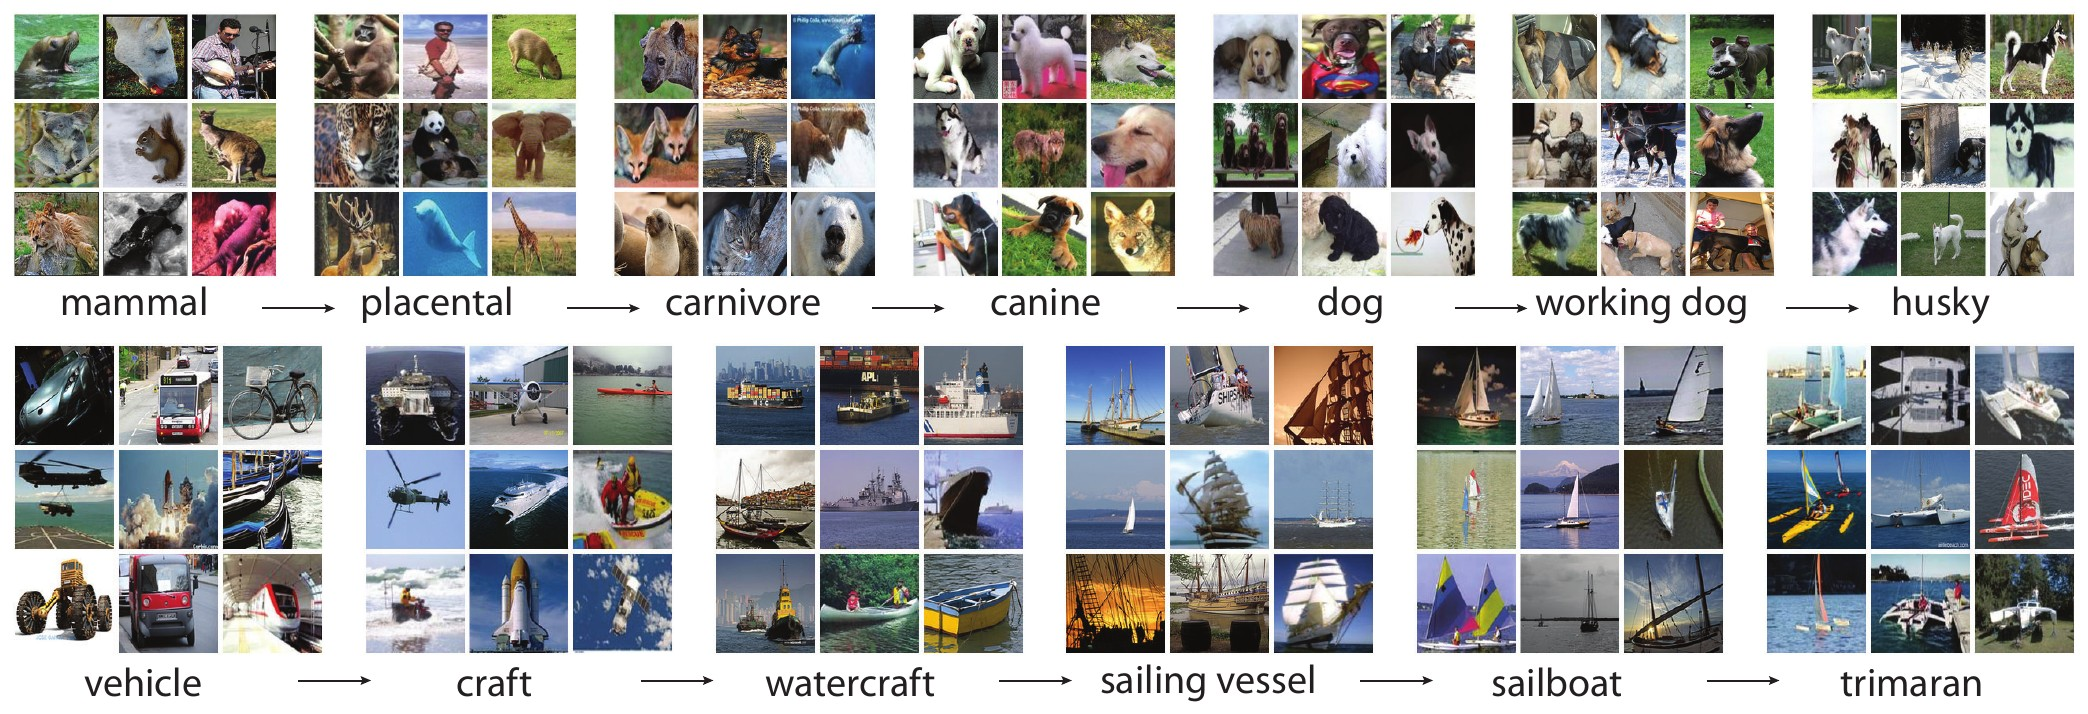
\includegraphics[width=0.93\linewidth]{imagenet_hierarchy.jpg}\end{center}
  \vskip -4pt
  {\scriptsize\color{gray} Two branches of the hierarchy, 9 random photos per category
  (Deng et al., "ImageNet", CVPR 2009, Fig. 1).}
  \vskip 3pt
  \small
  \textbf{22{,}000 categories}, taken from WordNet's tree of English nouns - from "mammal" all
  the way down to "husky". The yearly challenge used \textbf{1{,}000} of them, and \textbf{120
  are dog breeds}: telling a Siberian husky from a malamute counts.
  \vskip 3pt
  \fcolorbox{armred}{armred!8}{\parbox{0.97\linewidth}{\small
    Until 2011 the best programs got about \textbf{1 photo in 4 wrong} - even when allowed
    \textbf{five guesses}. Then something happened.}}
\end{frame}

% COLD OPEN
\begin{frame}{One chart, one question}
  \begin{center}
    \only<1>{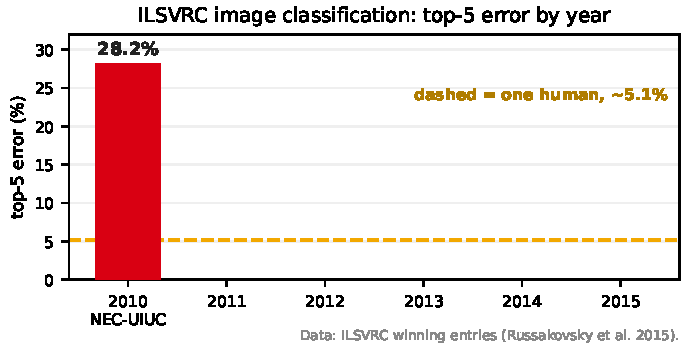
\includegraphics[width=4.3in]{imagenet_anim_1.pdf}}%
    \only<2>{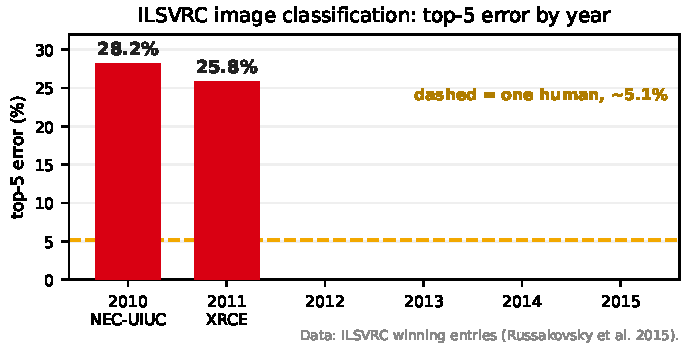
\includegraphics[width=4.3in]{imagenet_anim_2.pdf}}%
    \only<3>{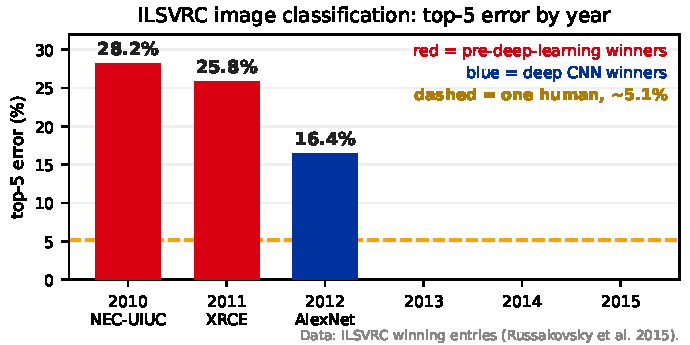
\includegraphics[width=4.3in]{imagenet_anim_3.pdf}}%
    \only<4>{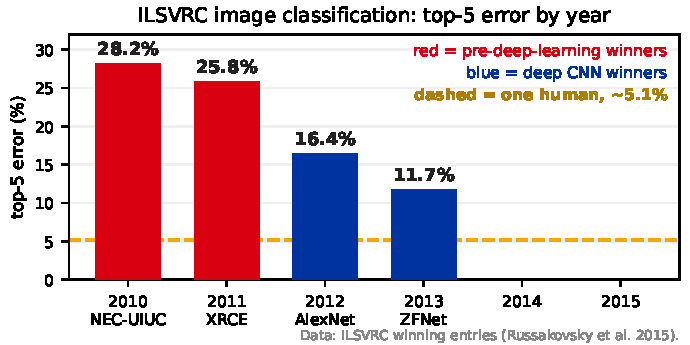
\includegraphics[width=4.3in]{imagenet_anim_4.pdf}}%
    \only<5>{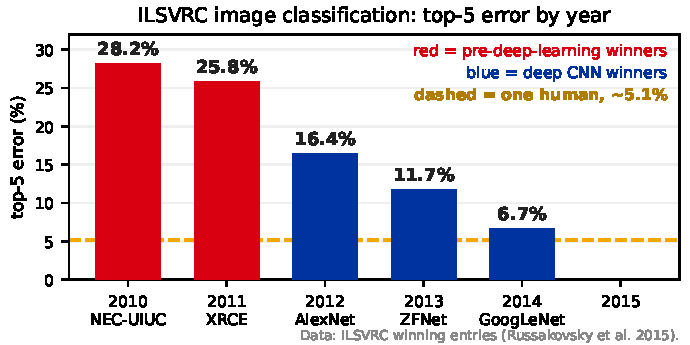
\includegraphics[width=4.3in]{imagenet_anim_5.pdf}}%
    \only<6>{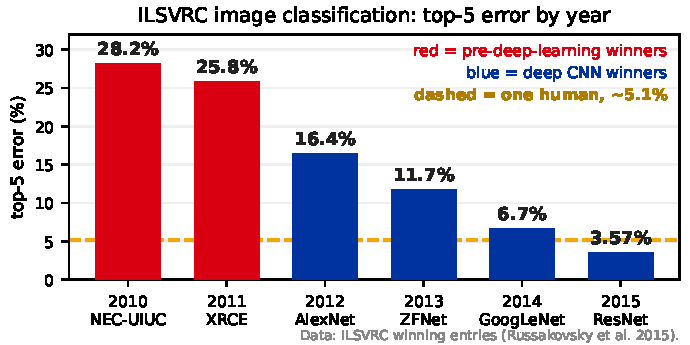
\includegraphics[width=4.3in]{imagenet_anim_6.pdf}}%
  \end{center}
  \vskip 1pt
  % fixed-height strip so the chart does not jump between clicks. One note per winner, shown
  % only on its own click (2026-10-02, instructor: notes for every year, pre-deep ones too).
  % Methods: Russakovsky et al., IJCV 2015 (2010 SIFT+LBP, non-linear coding, SVMs; 2011
  % compressed Fisher vectors, linear SVMs); the winners' papers for 2012-2015.
  \begin{minipage}[t][1.45cm][t]{\linewidth}\small
    \only<1>{\textcolor{armred}{\textbf{2010, NEC-UIUC}} (NEC Labs, Univ.\ of Illinois):
      hand-designed features (SIFT, LBP), encoded into one long vector, then linear SVMs.
      Experts designed the features - only the classifier learned.\par}
    \only<2>{\textcolor{armred}{\textbf{2011, XRCE}} (Xerox Research Europe): the same recipe
      with a better encoding of the hand-designed features (Fisher vectors), still linear SVMs.
      \textbf{Predict:} something happened in 2012. What?\par}
    \only<3>{\textcolor{armblue}{\textbf{2012, AlexNet}} (Toronto: Krizhevsky, Sutskever,
      Hinton) - the first deep CNN winner: 8 learned layers, 60 million weights, two gaming
      GPUs. Error $26\% \to 16\%$ in one year.\par}
    \only<4>{\textcolor{armblue}{\textbf{2013, ZFNet}} (Zeiler \& Fergus, NYU; entered as
      Clarifai): visualized what AlexNet's layers see, then fixed what looked broken - smaller
      first-layer filters ($7\times7$, stride 2).\par}
    \only<5>{\textcolor{armblue}{\textbf{2014, GoogLeNet}} (Google): 22 layers of Inception
      modules with 12$\times$ fewer weights than AlexNet. Runner-up VGG (Oxford, $7.3\%$) went
      deep with plain $3\times3$ stacks.\par}
    \only<6>{\fcolorbox{armblue}{armblue!8}{\parbox{0.97\linewidth}{\small
        \textcolor{armblue}{\textbf{2015, ResNet}} (Microsoft Research Asia): 152 layers,
        trainable thanks to skip connections - below one human's $5.1\%$. \textbf{Everything
        in this lecture is on this chart.}}}\par}
  \end{minipage}
\end{frame}

\begin{frame}{Outline}
  \tableofcontents
\end{frame}

% ================================================================
\section{The benchmark that made deep learning}

\begin{frame}[plain]
  \vfill
  \begin{center}
    {\Large\color{popblue}\textbf{ImageNet}}\\[0.9em]
    \begin{minipage}{0.82\textwidth}\centering\small
      Before the architectures, the arena: a dataset so large it changed what was worth building.
    \end{minipage}
  \end{center}
  \vfill
  \begin{center}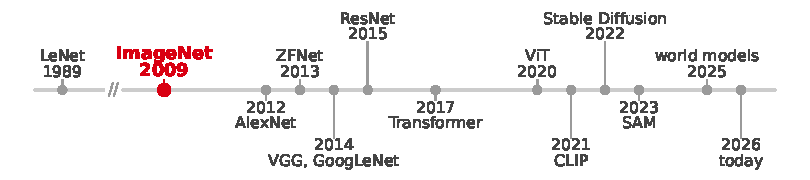
\includegraphics[width=5.4in]{ribbon_1.pdf}\end{center}
\end{frame}

\begin{frame}{The bet on data}
  In 2006, while most of computer vision tuned \textbf{algorithms}, \textbf{Fei-Fei Li}
  bet that what the field actually lacked was \textbf{data}.
  \vskip 6pt
  \begin{itemize}
    \item Built on \textbf{WordNet}'s noun hierarchy - with WordNet's creator,
      Christiane Fellbaum.
    \item Images scraped from the web; labeled by \textbf{Amazon Mechanical Turk}
      workers.
    \item Presented at CVPR \textbf{2009}, to little fanfare:
      \textbf{$\sim$14M labeled images}, $\sim$22{,}000 categories.
  \end{itemize}
  \vskip 8pt
  \fcolorbox{paramgreen}{paramgreen!8}{\parbox{0.97\linewidth}{\small
      The lesson that outlives every architecture in this deck: \textbf{data bets age
      better than algorithm bets}. Models come and go; ImageNet made all of them
      possible.}}
\end{frame}

\begin{frame}{ILSVRC and top-5 error}
  \begin{columns}[T]
    \column{0.52\textwidth}
    The annual \textbf{ImageNet Large Scale Visual Recognition Challenge} (ILSVRC)
    used a subset: \textbf{1.2M training images, 1{,}000 classes}.
    \vskip 6pt
    \textbf{Top-5 error}: the model proposes five labels; it is correct if the true
    label is among them - fair scoring when an image contains several things.
    \vskip 6pt
    \fcolorbox{armblue}{armblue!8}{\parbox{0.95\linewidth}{\small
      A shared benchmark accelerates a field for the same reason we always compare
      models on \emph{held-out} data ([06]): everyone measures the same thing, so
      progress is real and comparable.}}
    \column{0.48\textwidth}
    \begin{center}
      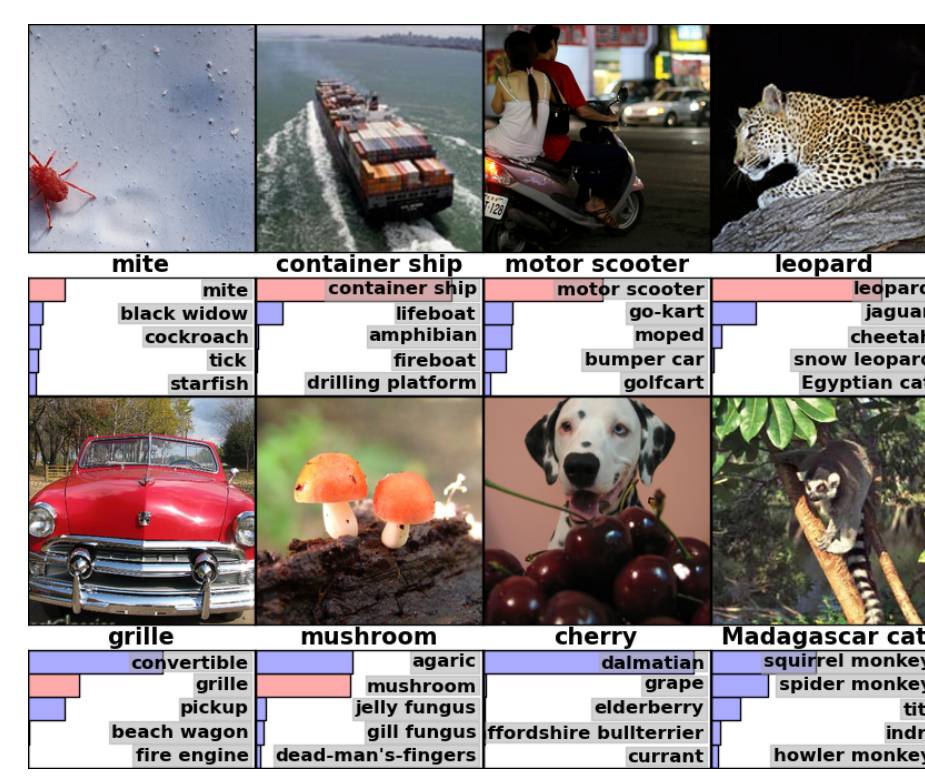
\includegraphics[width=0.86\linewidth]{imagenet_samples.png}\\[2pt]
      {\scriptsize AlexNet's five guesses per photo (ILSVRC-2010).
      \textcolor{armred}{\textbf{Red bar}} $=$ the correct label, if it made the top 5.}
    \end{center}
  \end{columns}
\end{frame}

% ================================================================
\section{The breakout: LeNet, AlexNet, ZFNet}

\begin{frame}[plain]
  \vfill
  \begin{center}
    {\Large\color{popblue}\textbf{The breakout}}\\[0.9em]
    \begin{minipage}{0.82\textwidth}\centering\small
      A blueprint from 1998, two gaming GPUs, and 1.2 million photos.
    \end{minipage}
  \end{center}
  \vfill
  \begin{center}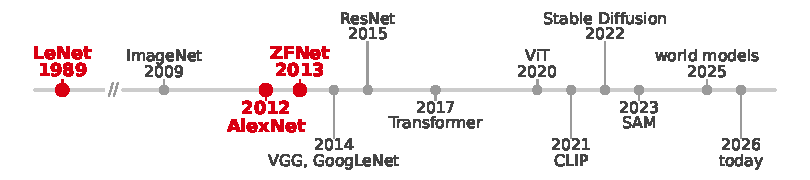
\includegraphics[width=5.4in]{ribbon_2.pdf}\end{center}
\end{frame}

\begin{frame}{LeNet (1998): the blueprint}
  \begin{columns}[T]
    \column{0.46\textwidth}
    \textbf{Yann LeCun}, AT\&T Bell Labs (joined 1988): backprop-trained
    convolutional nets reading \textbf{handwritten digits}.
    \vskip 4pt
    \texttt{conv-pool-conv-pool-dense}: everything in [48] was already here.
    \vskip 4pt
    Deployed commercially by NCR in \textbf{check-reading machines}; at its peak the
    system read an estimated \textbf{10-20\% of all checks} written in the US.
    \vskip 4pt
    Then the field moved on to SVMs, and CNNs went quiet for a decade. What was
    missing: \textbf{compute} and \textbf{data}.
    \column{0.54\textwidth}
    \begin{center}
      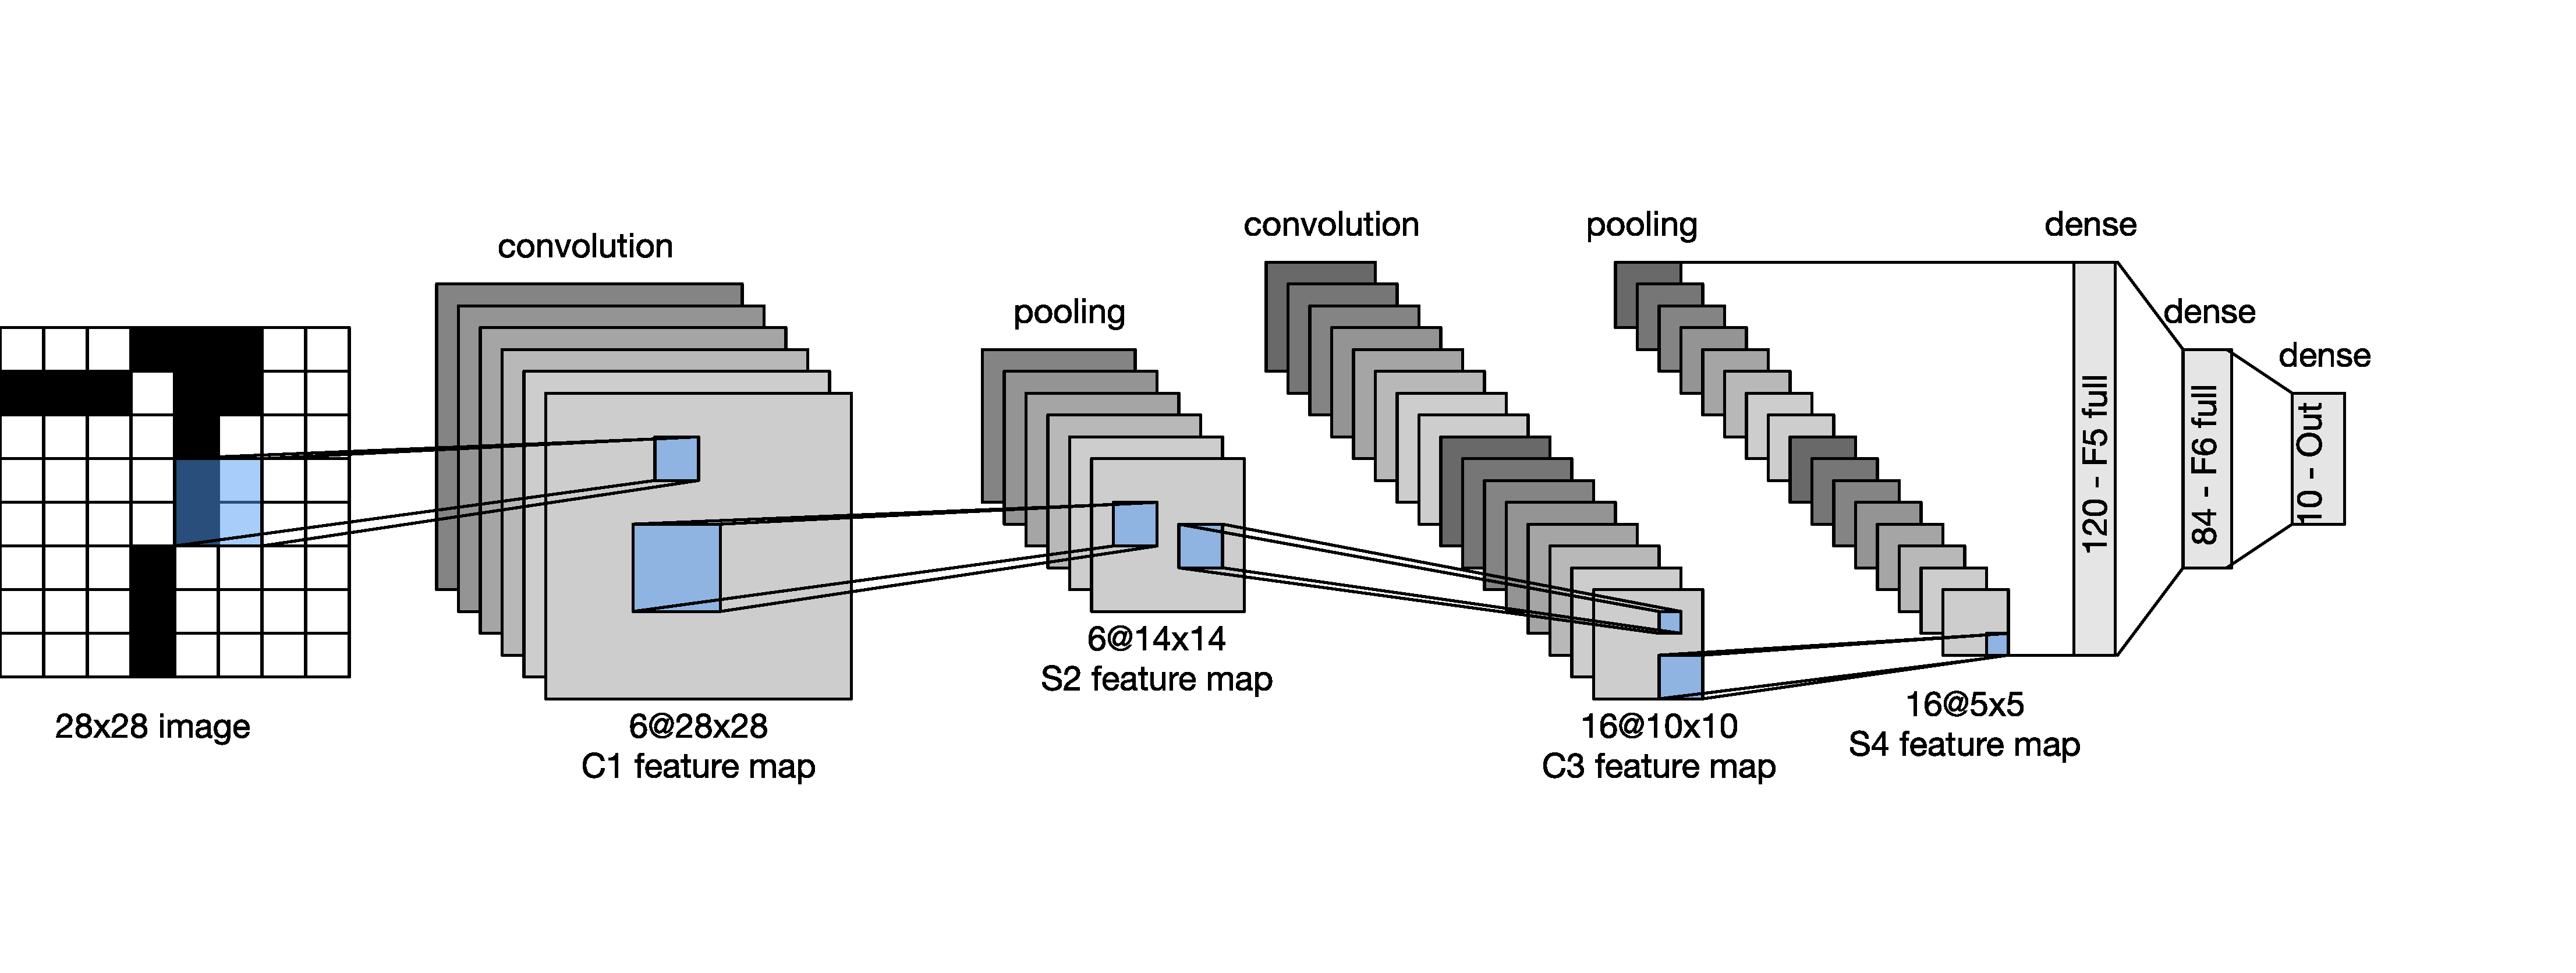
\includegraphics[width=\linewidth]{lenet_arch.pdf}
    \end{center}
    \vskip 4pt
    \begin{center}
      \href{https://adamharley.com/nn_vis/}{\beamergotobutton{play with a LeNet in 3D
      (Adam Harley)}}\;
      \href{https://poloclub.github.io/cnn-explainer/}{\beamergotobutton{CNN Explainer}}
    \end{center}
  \end{columns}
\end{frame}

\begin{frame}{AlexNet (2012): the breakout}
  \begin{columns}[T]
    \column{0.44\textwidth}
    Same blueprint, \textbf{scaled}: 8 layers, \textbf{60M parameters} - too big for
    one GPU, so Krizhevsky \textbf{split the network across two} consumer gaming
    cards (GTX 580, 3GB each) and trained \textbf{5-6 days} ($\sim$90 epochs over
    1.2M images) on a single PC.
    \vskip 4pt
    The GPU was the unlock: [42]'s hardware argument, made history.
    \vskip 4pt
    {\small Authors: Krizhevsky, Sutskever, Hinton (2012).}
    \column{0.56\textwidth}
    \begin{center}
      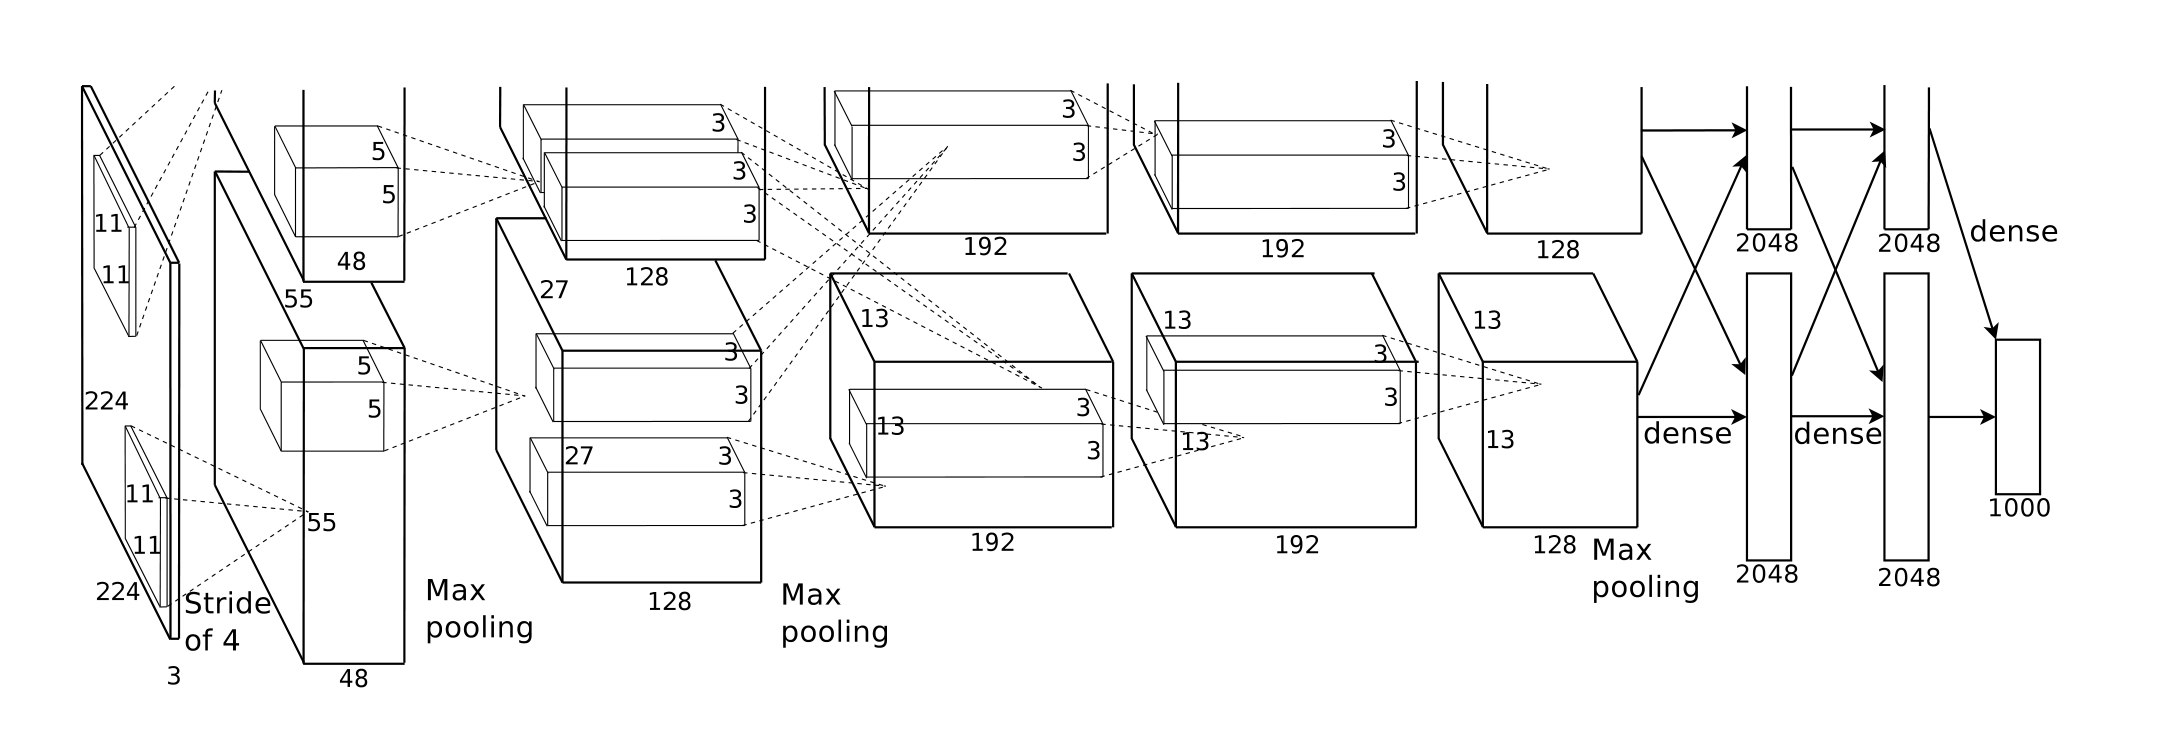
\includegraphics[width=\linewidth]{alexnet_twogpu.png}\\[1pt]
      {\scriptsize The paper's Figure 2, one GPU per half - cut off at the top in the
      published paper too.}
    \end{center}
    \vskip 2pt
    \fcolorbox{armblue}{armblue!8}{\parbox{0.95\linewidth}{\small
      The "new" tricks are all \textbf{[43]-[45] material deployed at once}: ReLU
      instead of saturating tanh (the paper's test net hit 25\% training error
      \textbf{6$\times$ faster}), dropout, data augmentation. You already know every
      ingredient - they had the hardware to use them at scale.}}
  \end{columns}
\end{frame}

% 2026-10-01 (l17_todo #5, "facts like AlexNet"). 15.3 vs 26.2: ILSVRC 2012 results (runner-up
% = best non-neural entry). cuda-convnet: Krizhevsky's own GPU library. DNNresearch auction at
% NIPS 2012, Lake Tahoe, $44M to Google (Wired 2021; U of T release 2013). CHM + Google released
% the original code, March 2025. Rank 8: Nature, April 2025. All web-checked 2026-10-01.
\begin{frame}{AlexNet: the rest of the story}
  \begin{itemize}
    \item \textbf{The margin.} $15.3\%$ top-5 error against $26.2\%$ for the runner-up - a
      lead of almost 11 points in a contest usually won by one or two.
    \item \textbf{Home-made software.} Krizhevsky wrote his own GPU code (cuda-convnet) to fit
      the training into a week.
    \item \textbf{The auction.} Hinton and his two students formed a company, DNNresearch, and
      auctioned it at the NIPS conference in Lake Tahoe that December. Big tech companies bid;
      Hinton stopped at \textbf{\$44M} and sold to Google.
    \item \textbf{The code.} In 2025 the Computer History Museum and Google published AlexNet's
      original source code on GitHub.
    \item \textbf{The citations.} The 8th most-cited paper of the 21st century, across all of
      science (Nature, 2025).
  \end{itemize}
  \vskip 6pt
  \fcolorbox{paramgreen}{paramgreen!8}{\parbox{0.97\linewidth}{\small
    AlexNet invented almost none of its parts - they were LeNet's blueprint plus [43]-[45]. What
    it proved is that they \textbf{scale}.}}
\end{frame}

% 2026-10-01 (l17_todo #1): Welch Labs, "The moment we stopped understanding AI [AlexNet]",
% 2024-07-01, 17:38. Still = _reference_welchlabs_alexnet/frames/f02_00-04-30.jpg (AlexNet's
% first-layer filters) -> fig/borrowed/welchlabs_alexnet_filters.jpg.
\mustwatch{welchlabs_alexnet_filters.jpg}{Welch Labs, 2024}{https://www.youtube.com/watch?v=UZDiGooFs54}{The moment we stopped understanding AI [AlexNet]}{18 minutes: what AlexNet's layers learned, from these first-layer filters to activation atlases.}

% 2026-10-01 (l17_todo #5). Facts from Zeiler & Fergus, arXiv 1311.2901 (ECCV 2014), Sec. 4.1 and
% Fig. 6: AlexNet's layer-1 filters "a mix of extremely high and low frequency information" with
% dead features; layer-2 aliasing from stride 4 -> 7x7, stride 2. Clarifai 11.7% (ILSVRC 2013,
% GoogLeNet paper Table 2). Image: their Fig. 2 (fig/borrowed/zfnet_layers.jpg).
\begin{frame}{ZFNet (2013): look inside, then fix it}
  \begin{columns}[T]
    \column{0.62\textwidth}
    \small
    \textbf{Matthew Zeiler} and \textbf{Rob Fergus} (NYU) asked what each layer of AlexNet
    responds to. Their \textbf{deconvnet} runs a feature map backwards to the pixels that
    excited it (right: layers 1 to 5, each with the image patches that fire it most).
    \vskip 4pt
    What they saw in AlexNet: first-layer filters that were only very coarse or very fine, some
    of them dead, and \textbf{aliasing} in layer 2 from the huge $11\times11$, stride-4 first
    convolution. The fix: $7\times7$ with stride 2 - and accuracy went up.
    \vskip 4pt
    Zeiler's startup \textbf{Clarifai} won ILSVRC 2013 with this design: \textbf{11.7\%}.
    \vskip 4pt
    \fcolorbox{armblue}{armblue!8}{\parbox{0.95\linewidth}{\small
      Visualization as a \textbf{debugging tool}: look at what the network learned, then change
      the architecture. [50]'s Grad-CAM is the same idea.}}
    \column{0.36\textwidth}
    \begin{center}
      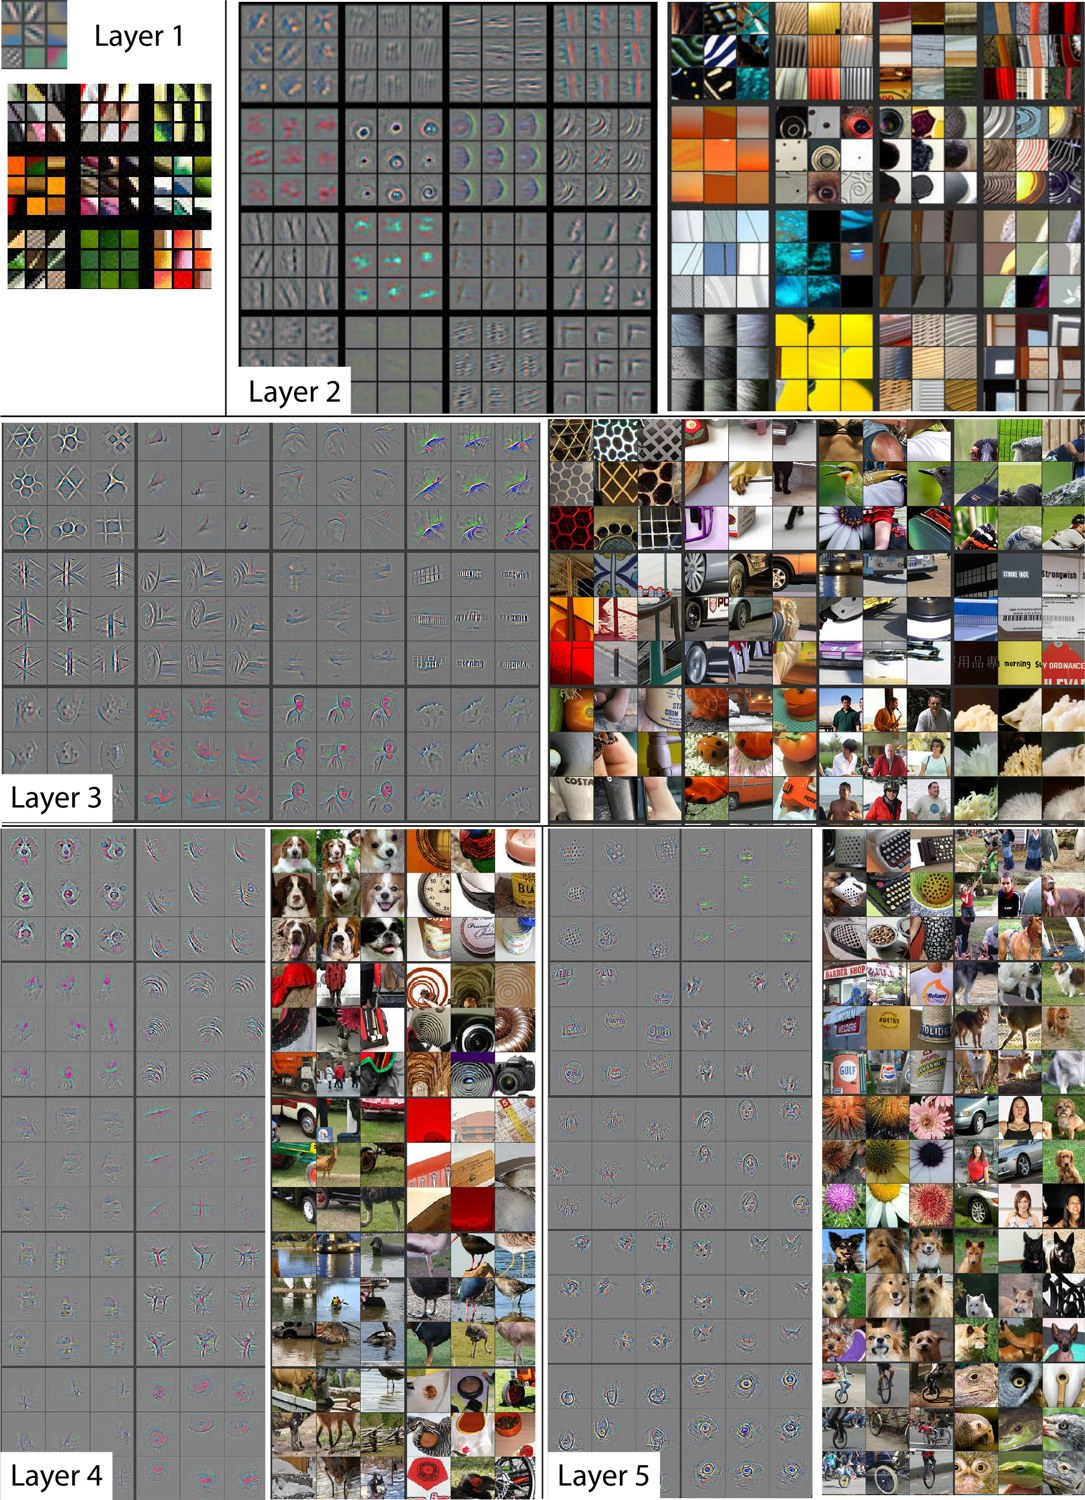
\includegraphics[height=0.72\textheight]{zfnet_layers.jpg}\\[1pt]
      {\scriptsize Zeiler \& Fergus, ECCV 2014, Fig. 2}
    \end{center}
  \end{columns}
\end{frame}

\begin{frame}{What AlexNet-style networks learn}
  \begin{columns}[T]
    \column{0.40\textwidth}
    First-layer filters of a modern pretrained network (ResNet-18, trained on
    ImageNet): crisp \textbf{Gabor-like edge, blob and color detectors}.
    \vskip 6pt
    The \textbf{[48] kernel zoo} - reinvented by gradient descent, designed by
    nobody.
    \vskip 6pt
    \fcolorbox{armblue}{armblue!8}{\parbox{0.95\linewidth}{\small
      [48]'s tiny Fashion-MNIST kernels looked blurry; at ImageNet scale the learned
      kernels become \emph{textbook}. The hand-designed $\to$ learned arc closes
      here.}}
    \column{0.60\textwidth}
    \begin{center}
      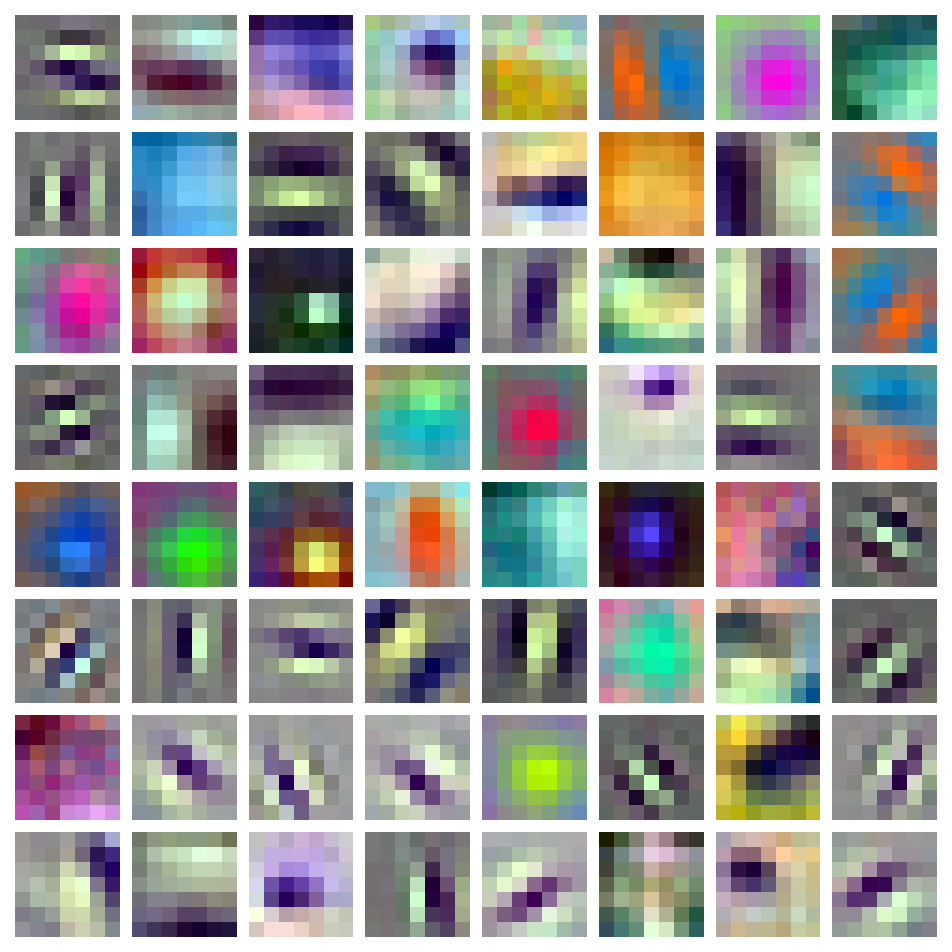
\includegraphics[height=0.70\textheight]{pretrained_filters.pdf}\\[1pt]
      {\scriptsize ResNet-18's 64 first-layer filters ($7\times7$, RGB)}
    \end{center}
  \end{columns}
\end{frame}

% ================================================================
\section{2014: deeper, or wider?}

\begin{frame}[plain]
  \vfill
  \begin{center}
    {\Large\color{popblue}\textbf{2014: deeper, or wider?}}\\[0.9em]
    \begin{minipage}{0.82\textwidth}\centering\small
      Two answers in one year: stack small filters (VGG), or run several filter sizes side by side (GoogLeNet).
    \end{minipage}
  \end{center}
  \vfill
  \begin{center}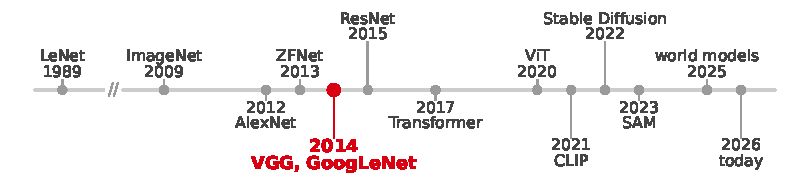
\includegraphics[width=5.4in]{ribbon_3.pdf}\end{center}
\end{frame}

% 2026-10-01 (l17_todo #9): the receptive field now comes BEFORE VGG, because VGG's argument
% depends on it. Figure: receptive_field.py (nested fields only, drawn at slide size).
\begin{frame}{Receptive field: how far a neuron sees}
  \begin{columns}[T]
    \column{0.44\textwidth}
    \small
    The \textbf{receptive field} of a neuron is the patch of the \emph{input image} that can
    influence it.
    \vskip 4pt
    One $3\times3$ conv: each output sees $3\times3$ pixels. Put a second $3\times3$ conv on top:
    each of \emph{its} outputs sees $3\times3$ outputs of the first - and together those cover
    $5\times5$ pixels. A third layer: $7\times7$.
    \vskip 4pt
    Early layers see \emph{edges}; deep layers see \emph{objects} - [48]'s feature hierarchy,
    measured in pixels.
    \column{0.54\textwidth}
    \begin{center}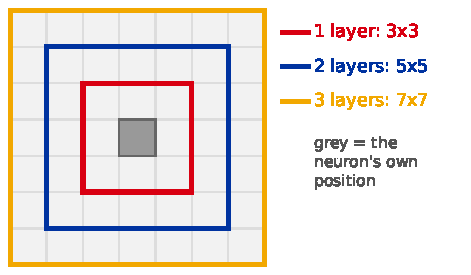
\includegraphics[width=\linewidth]{receptive_field.pdf}\end{center}
  \end{columns}
  \vskip 4pt
  \fcolorbox{armblue}{armblue!8}{\parbox{0.97\linewidth}{\small
    Every extra $3\times3$ layer adds 2 pixels of reach. (Reach \emph{without} more layers: [48]'s
    dilated convolutions, back in [51].)}}
\end{frame}

% 2026-10-01 (l17_todo #9, "VGG - I didn't get it"): the argument now uses the receptive-field
% frame's numbers (VGG paper, Sec. 2.3: three 3x3 = 27 C^2 vs one 7x7 = 49 C^2, "81% more").
% 49*64^2 = 200,704; 27*64^2 = 110,592; 1 - 27/49 = 45% fewer.
\begin{frame}{VGG (2014): small filters, stacked}
  \small
  So three stacked $3\times3$ layers see what \textbf{one} $7\times7$ layer sees. \textbf{Which
  costs fewer weights?} (Each layer: $C$ channels in, $C$ out; biases ignored.)
  \pause
  \vskip 6pt
  \begin{columns}[T]
    \column{0.56\textwidth}
    \begin{center}
      \begin{tabular}{l c c}
        & \textbf{one} $7\times7$ & \textbf{three} $3\times3$\\
        \hline
        sees & $7\times7$ & $7\times7$\\
        weights & $49\,C^2$ & $3\cdot9\,C^2 = 27\,C^2$\\
        at $C = 64$ & $200{,}704$ & $110{,}592$\\
        nonlinearities & 1 ReLU & 3 ReLUs\\
      \end{tabular}
    \end{center}
    \vskip 6pt
    \fcolorbox{armblue}{armblue!8}{\parbox{0.95\linewidth}{\small
      Same view, \textbf{45\% fewer weights}, and three nonlinearities instead of one. That one
      observation is the whole VGG design.}}
    \column{0.42\textwidth}
    \begin{center}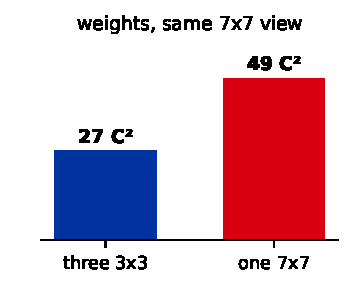
\includegraphics[width=2.3in]{vgg_cost.pdf}\end{center}
  \end{columns}
\end{frame}

% 2026-10-01: vgg_layout.py (block weights computed, total checked against torchvision vgg16:
% 138,357,544; dense 123,642,856). VGG 2014: 7.32% top-5 (2nd), 1st in localization.
\begin{frame}{VGG-16, layer by layer}
  \small
  Repeat the trick: blocks of $3\times3$ convs, a $2\times2$ max-pool after each block, and
  \textbf{twice the channels} each time the grid halves.
  \vskip 2pt
  \begin{center}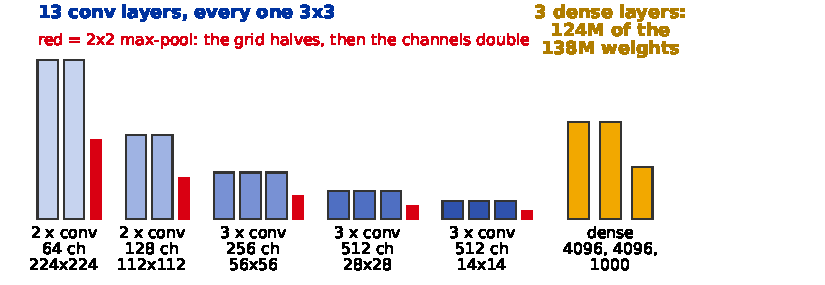
\includegraphics[width=5.1in]{vgg_layout.pdf}\end{center}
  \vskip 2pt
  \begin{itemize}\small
    \item 2nd in 2014 ($7.3\%$). Simple and uniform, so it became the favourite
      \textbf{feature extractor} - [51]'s style transfer runs on VGG.
    \item But the three dense layers hold \textbf{124M of the 138M} weights. Hold that thought.
  \end{itemize}
\end{frame}

\begin{frame}{Who built VGG}
  \textbf{Karen Simonyan} and Andrew Zisserman, Oxford's \textbf{V}isual
  \textbf{G}eometry \textbf{G}roup - and yes, Karen Simonyan is an Armenian name.
  \vskip 8pt
  His arc since:
  \begin{itemize}
    \item \textbf{DeepMind} (2014-2022) - contributor to AlphaZero, AlphaFold,
      WaveNet;
    \item co-founder of \textbf{Inflection AI} (2022, with Reid Hoffman and Mustafa
      Suleyman);
    \item now \textbf{Chief Scientist at Microsoft AI}.
  \end{itemize}
  \vskip 8pt
  \fcolorbox{paramgreen}{paramgreen!8}{\parbox{0.97\linewidth}{\small
      A VGG author's career \emph{is} the last decade of AI in miniature: benchmark
      vision $\to$ deep-learning lab $\to$ startup $\to$ big-tech frontier lab.}}
\end{frame}

\begin{frame}{$1\times1$ convolutions}
  A $1\times1$ conv is a \textbf{per-pixel dense layer across channels}: it mixes
  \emph{depth} without touching \emph{space}.
  \vskip 4pt
  Two jobs:
  \begin{enumerate}
    \item \textbf{cheap channel reduction} before expensive convolutions,
    \item an extra \textbf{nonlinearity} almost for free.
  \end{enumerate}
  \vskip 6pt
  Reduce $256 \to 64$ channels:
  \[
    1{\times}1:\ 256 \cdot 64 + 64 = \mathbf{16{,}448}
    \qquad\text{vs}\qquad
    3{\times}3:\ 9 \cdot 256 \cdot 64 + 64 = \mathbf{147{,}520}
  \]
  \vskip 4pt
  \fcolorbox{paramgreen}{paramgreen!8}{\parbox{0.97\linewidth}{\small
      Pointwise convolutions return in [51] (separable convolutions - how phones
      afford CNNs).}}
\end{frame}

\begin{frame}{The Inception block}
  \begin{columns}[T]
    \column{0.40\textwidth}
    Why choose a kernel size at all? Run $1\times1$, $3\times3$, $5\times5$
    \textbf{and} a pooling path \textbf{in parallel}, and \textbf{concatenate} the
    maps.
    \vskip 6pt
    The network picks its own mix, layer by layer.
    \vskip 6pt
    \fcolorbox{armblue}{armblue!8}{\parbox{0.95\linewidth}{\small
      The $1\times1$ bottlenecks (white boxes) are what keep four parallel paths
      \emph{affordable} - the previous slide's trick, deployed.}}
    \column{0.60\textwidth}
    \begin{center}
      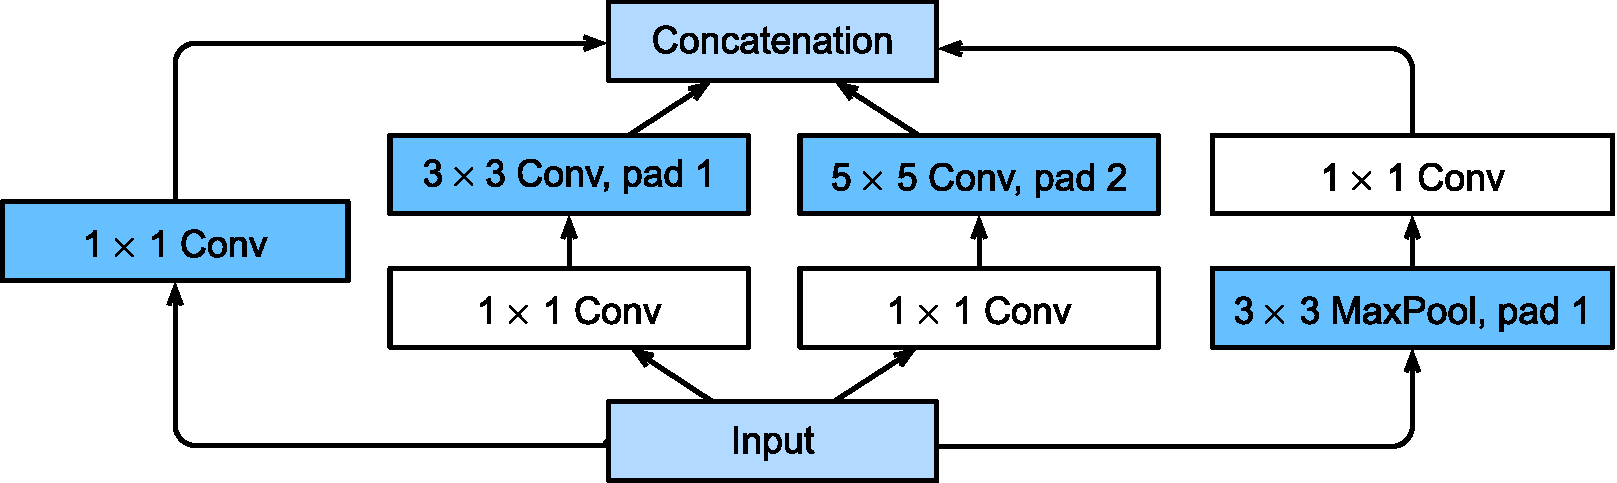
\includegraphics[width=\linewidth]{inception_block.pdf}
    \end{center}
  \end{columns}
\end{frame}

% 2026-10-01 (l17_todo #5): facts from Szegedy et al., arXiv 1409.4842: 22 layers with
% parameters (27 with pooling); "homage to Yann LeCun's pioneering LeNet 5"; "Inception" from
% Network-in-Network + the "we need to go deeper" meme (reference [1]); CPU-only training
% (DistBelief); 6.67% top-5, ensemble of 7.
\begin{frame}{GoogLeNet (2014): a network of Inception blocks}
  The \textbf{2014 winner}, from Google: Inception blocks stacked \textbf{22 layers} deep -
  \textbf{6.7\%} top-5 error with \textbf{under 7M parameters} (AlexNet: 60M).
  \vskip 2pt
  \begin{center}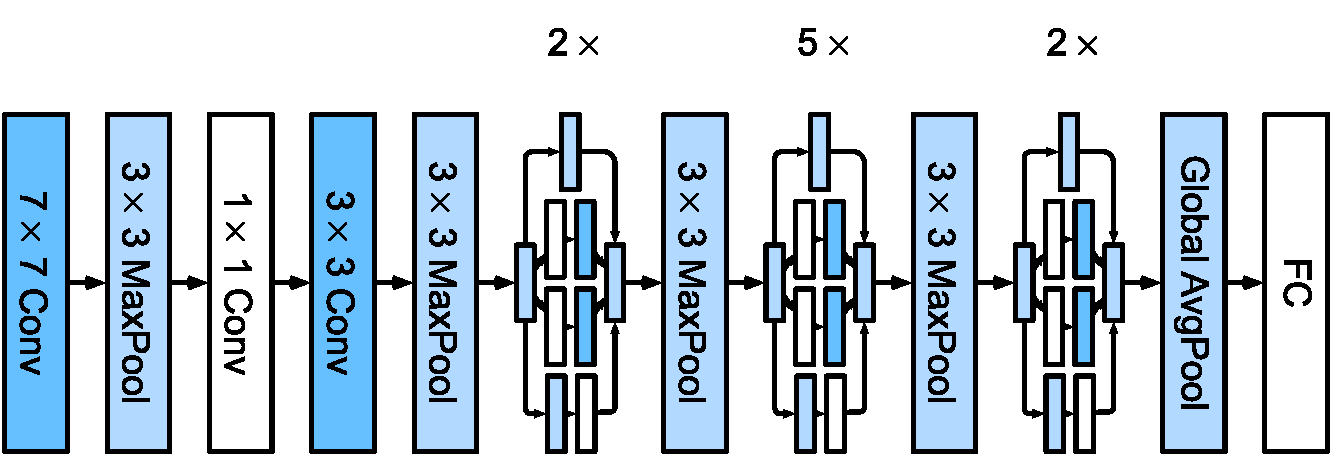
\includegraphics[width=0.82\linewidth]{googlenet_full.pdf}\end{center}
  \vskip 2pt
  \begin{columns}[T]
    \column{0.49\textwidth}
    \fcolorbox{armorange}{armorange!12}{\parbox{0.95\linewidth}{\scriptsize
      \textbf{The names.} "GoogLeNet" - capital L - is an homage to LeCun's LeNet.
      "Inception" is the film meme "we need to go deeper"; the paper cites it as reference
      [1].}}
    \column{0.49\textwidth}
    \fcolorbox{armblue}{armblue!8}{\parbox{0.95\linewidth}{\scriptsize
      No giant dense head: it ends in a \emph{global average pool} (in two slides). And it was
      trained on \textbf{CPUs only}, on Google's distributed system.}}
  \end{columns}
\end{frame}

% 2026-10-01 (l17_todo #3): Carter, Armstrong, Schubert, Johnson & Olah, "Activation Atlas",
% Distill 2019 (CC BY 4.0). Image = the repo's render of InceptionV1 (= GoogLeNet) layer mixed4c,
% 1M sample images, UMAP layout (filename: sample_images=1000000, layout=50_0.05_cosine),
% downscaled to 1200 px -> fig/borrowed/distill_activation_atlas_mixed4c.jpg.
\begin{frame}{What GoogLeNet sees: an activation atlas}
  \begin{columns}[T]
    \column{0.50\textwidth}
    \small
    Push a \textbf{million images} through GoogLeNet and record one layer's activations
    (mixed4c: 512 numbers per image patch).
    \vskip 3pt
    Lay the million vectors out in 2D so that \textbf{similar activations land close together}
    (UMAP, from the dimensionality-reduction chapter), average each grid cell, and render each
    average with feature visualization ([48]).
    \vskip 3pt
    The result is a map of what that layer can represent: \textbf{animal faces} top left,
    \textbf{people} top right, \textbf{plants} on the left, \textbf{water and landscapes} at the
    bottom, \textbf{buildings and objects} on the right.
    \vskip 4pt
    \href{https://distill.pub/2019/activation-atlas/}{\beamergotobutton{explore it:
    distill.pub/2019/activation-atlas}}
    \column{0.48\textwidth}
    \begin{center}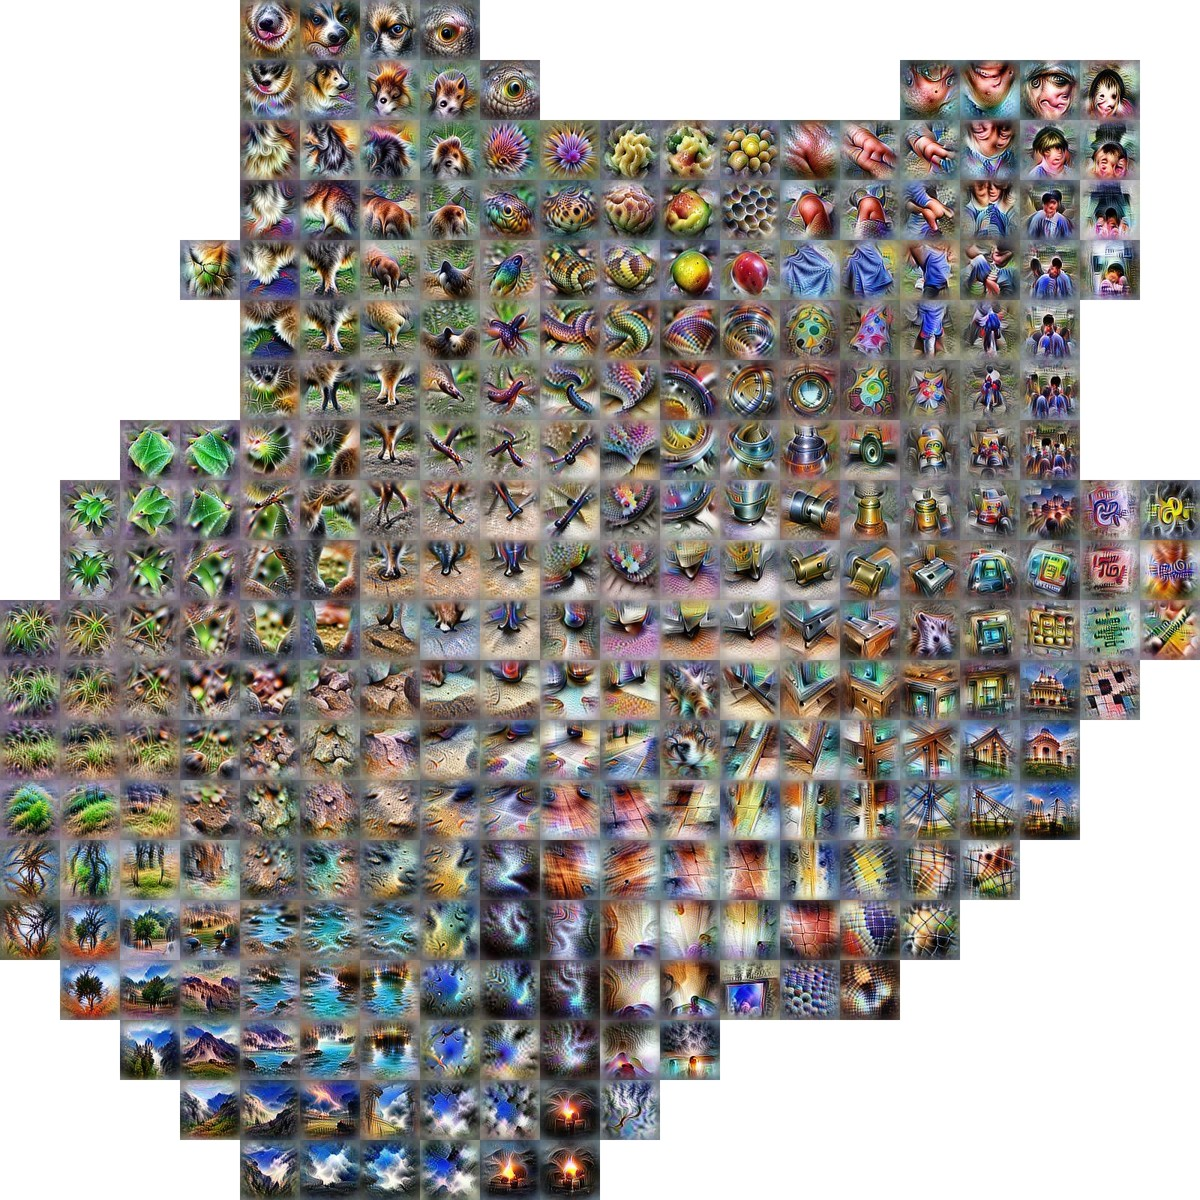
\includegraphics[height=0.80\textheight]{distill_activation_atlas_mixed4c.jpg}\end{center}
  \end{columns}
  \vskip -2pt
  {\scriptsize\color{gray} Carter, Armstrong, Schubert, Johnson \& Olah, "Activation Atlas",
  Distill (2019), CC BY 4.0.}
\end{frame}

\begin{frame}{The dense-head problem}
  \textbf{Predict first:} AlexNet has 60M parameters. Where do \emph{most} of them
  live - the conv layers, or somewhere else?
  \pause
  \vskip 6pt
  \fcolorbox{armred}{armred!8}{\parbox{0.97\linewidth}{\small
      In the \textbf{flatten $\to$ dense head}. AlexNet's dense layers hold roughly
      \textbf{58 of its 60M} weights; VGG-16's, \textbf{124M of 138M}.}}
  \vskip 6pt
  Why: flattening keeps every pixel of every map. Take a modest final stack of
  \textbf{256 maps of $100\times100$}, into a 10-class dense layer:
  \[
    256 \cdot 100 \cdot 100 \cdot 10 = \mathbf{25{,}600{,}000}\ \text{weights}
  \]
  \vskip 2pt
  More than all the conv layers combined - spent on one classification layer.
\end{frame}

\begin{frame}{Global average pooling}
  The fix (from Network-in-Network), \textbf{global average pooling} (GAP):
  \textbf{average each final map to one number}. 256 maps $\to$ a 256-vector $\to$ dense-10.
  \vskip 4pt
  \textbf{Compute the head's weight count yourself.}
  \pause
  \[
    256 \cdot 10 = \mathbf{2{,}560}\ \text{weights}
    \qquad\text{(was } 25{,}600{,}000\text{)} - \text{a } \mathbf{10{,}000\times}
    \text{ cut}
  \]
  \vskip 4pt
  Bonus: GAP acts as a \textbf{regularizer} (no giant head to overfit) and accepts
  \textbf{any input size} (the average does not care how big the map is). Why average,
  not max? Global max pooling exists; the average uses every location's evidence and
  spreads the gradient over all of them, so it became the default.
  \vskip 6pt
  \fcolorbox{paramgreen}{paramgreen!8}{\parbox{0.97\linewidth}{\small
      The \textbf{[48] pooling} operation with a \emph{global} window. Used by
      everything modern - ResNet already ends this way.}}
\end{frame}

% 2026-10-01 addition (instructor-approved): the Gesture Snake practical's known-answer test
% (DECISIONS #57). 1,000 synthetic crops (disc + bar in the labelled direction, or no bar),
% same small-CNN body, augmentation on: flatten head 77.2%, GAP head 24.6%, frozen ResNet-18
% features + logistic regression 99.6%. Receptive field of the small net's final features,
% computed layer by layer (avgpool 2, then 3x [conv3 + maxpool2]): 44 px of the 128 px crop.
\begin{frame}{When averaging away \emph{where} hurts}
  \small
  The chapter's practical, Gesture Snake, asks: \textbf{which way does the thumb point?}
  (up, down, left, right, or no thumb). A known-answer test: 1{,}000 synthetic crops, a disc
  (the fist) with a bar (the thumb) on one side. One small CNN body - three conv blocks down to
  64 maps of $8\times8$ - with two different heads. \textbf{Predict:} does GAP still win?
  \pause
  \vskip 4pt
  \begin{columns}[T]
    \column{0.46\textwidth}
    \begin{center}\footnotesize
      \begin{tabular}{l r}
        \textbf{model} & \textbf{held-out acc.}\\
        \hline
        small CNN $+$ flatten head & $77\%$\\
        small CNN $+$ GAP head & $\mathbf{25\%}$\\
        pretrained ResNet-18 & \\
        \quad (ends in GAP) $+$ linear head & $99.6\%$\\
        \hline
        guessing, 5 classes & $20\%$\\
      \end{tabular}
    \end{center}
    \column{0.52\textwidth}
    \fcolorbox{armorange}{armorange!12}{\parbox{0.95\linewidth}{\small
      A horizontal bar looks the same pointing left or right - the answer is which
      \emph{side} of the disc it sits on. This net's final features each see only about a
      third of the crop, so the side lives in their \emph{position} in the $8\times8$ map -
      and GAP averages position away.}}
  \end{columns}
  \vskip 4pt
  \fcolorbox{paramgreen}{paramgreen!8}{\parbox{0.97\linewidth}{\small
    ResNet-18 averages too, yet scores $99.6\%$: its final features each see the
    \textbf{whole} crop, so "which side" is computed \emph{before} the average. GAP is safe
    once the \textbf{receptive field covers the object}; before that, flatten - or go deeper.}}
  \vskip 2pt
  {\scriptsize\color{gray} Synthetic stand-in images, measured while building the practical
  (the notebook itself trains on your own photos).}
\end{frame}

% ================================================================
\section{2015: ResNet}

\begin{frame}[plain]
  \vfill
  \begin{center}
    {\Large\color{popblue}\textbf{If depth is good, why not 100 layers?}}\\[0.9em]
    \begin{minipage}{0.82\textwidth}\centering\small
      Because past $\sim$20 layers, plain networks get \emph{worse} - and the fix reshaped every deep network since.
    \end{minipage}
  \end{center}
  \vfill
  \begin{center}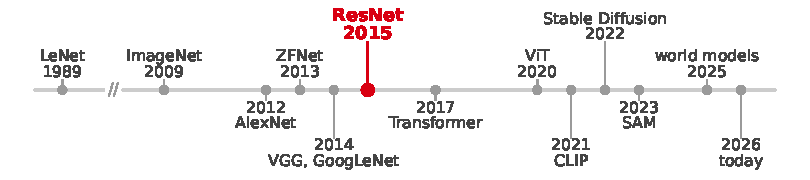
\includegraphics[width=5.4in]{ribbon_4.pdf}\end{center}
\end{frame}

\begin{frame}{Predict first: the degradation problem}
  A \textbf{56-layer} plain net vs a \textbf{20-layer} plain net - same data, same
  recipe. \textbf{Which one has lower \emph{training} error?}
  \pause
  \vskip 4pt
  \begin{center}
    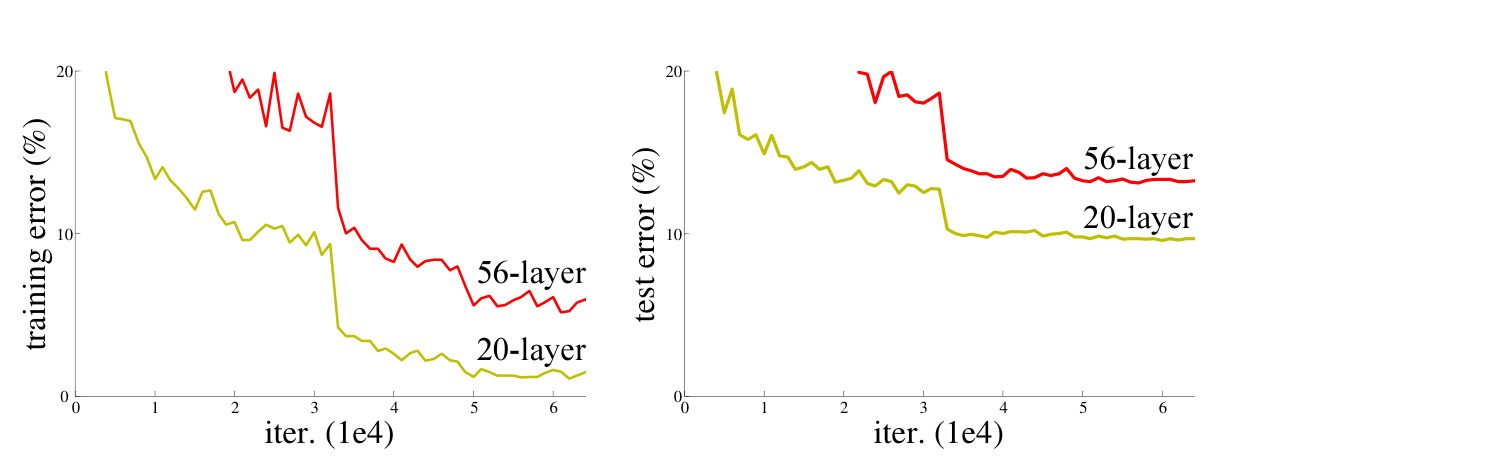
\includegraphics[width=0.72\linewidth]{he_degradation.png}
  \end{center}
  \vskip 2pt
  \fcolorbox{armred}{armred!8}{\parbox{0.97\linewidth}{\small
      \textbf{The 20-layer one} (He et al. 2015, Figure 1). This is \emph{not}
      overfitting - it is \emph{training} error. Deep plain nets are simply
      \textbf{hard to optimize}: the deeper model could imitate the shallow one by
      making 36 layers do nothing, yet gradient descent fails to find even that.
      "Do nothing" is a precise target for conv+ReLU layers - every weight must line
      up so the input comes out unchanged, and nothing pulls a random start there.}}
\end{frame}

\begin{frame}{The residual idea}
  \begin{columns}[T]
    \column{0.47\textwidth}
    Let the block learn the \textbf{correction}, not the whole mapping:
    \vskip 4pt
    \fcolorbox{popblue}{popblue!6}{\parbox{0.9\linewidth}{\centering
      $H(\xv) = F(\xv) + \xv$}}
    \vskip 6pt
    The \textbf{skip connection} carries $\xv$ for free; the layers only learn the
    residual $F(\xv)$.
    \vskip 6pt
    Learning "do nothing" is now trivial - push $F \to 0$ - so \textbf{extra layers
    can no longer hurt}.
    \vskip 6pt
    {\small If dimensions change, project the shortcut:
    $H(\xv) = F(\xv) + W_s\,\xv$.}
    \column{0.53\textwidth}
    \begin{center}
      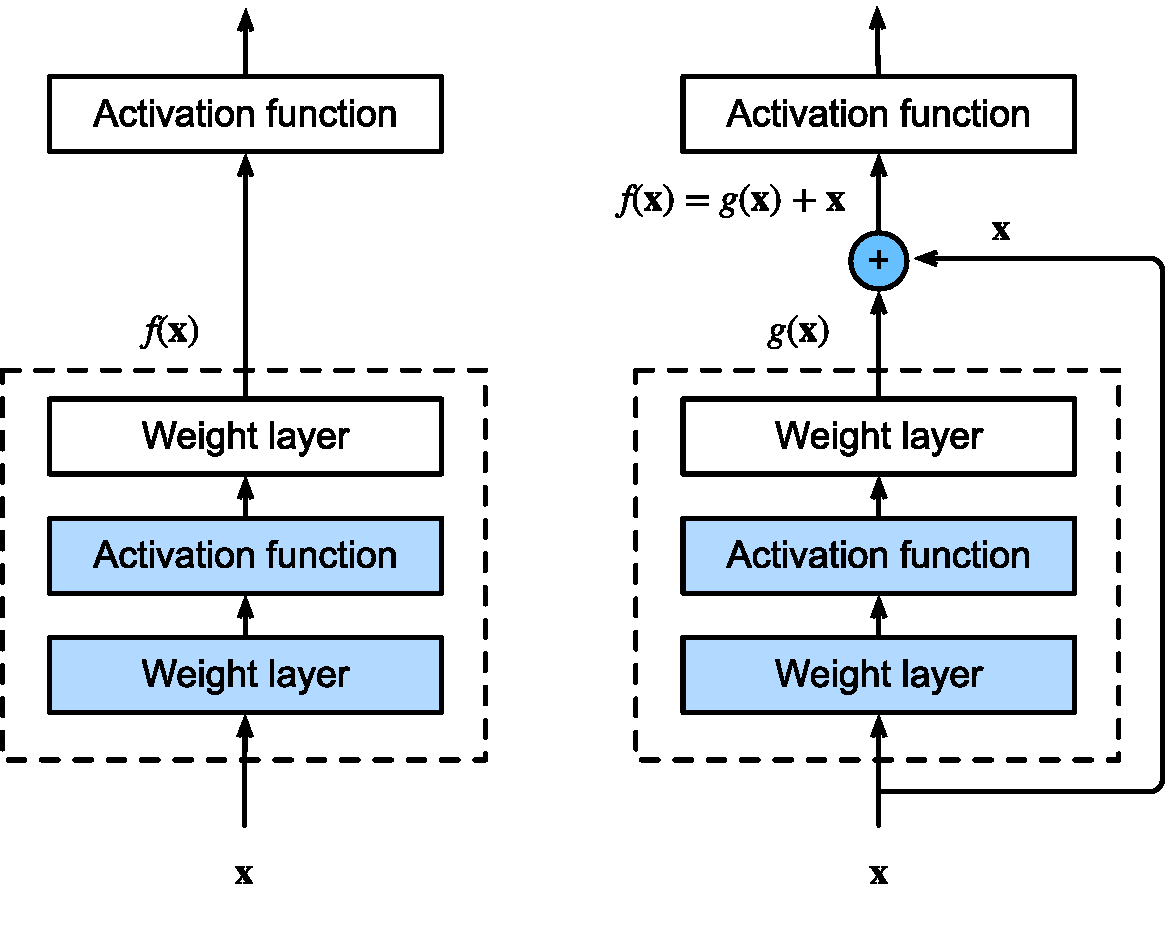
\includegraphics[height=0.62\textheight]{residual_block.pdf}\\[1pt]
      {\scriptsize Left: a plain block must learn all of $f(\mathbf{x})$.
       Right: a residual block only learns the difference $g(\mathbf{x})$.}
    \end{center}
  \end{columns}
\end{frame}

\begin{frame}{You have seen residual learning before}
  \begin{center}
    {\large $H(\xv) = F(\xv) + \xv$}
  \end{center}
  \vskip 4pt
  \textbf{Recall:} where in this course have you already met a model that only fits
  a \textbf{correction} to what already exists?
  \pause
  \vskip 6pt
  \fcolorbox{armblue}{armblue!8}{\parbox{0.97\linewidth}{
      \textbf{Gradient boosting} (ch4): every new tree fits the \emph{residual} of
      the ensemble so far. A ResNet block does the same thing \textbf{in depth} -
      boosting stacks residual learners in sequence, ResNet stacks them layer on
      layer.}}
  \vskip 6pt
  \fcolorbox{armorange}{armorange!12}{\parbox{0.97\linewidth}{\small
      Analogy, not identity: boosting fits each learner to the \emph{frozen}
      ensemble's residual, stage by stage; ResNet blocks train \emph{jointly}, end
      to end.}}
\end{frame}

\begin{frame}{Why skips also fix gradients}
  The identity path is not just easy to learn - it is an \textbf{undamped route for
  the gradient} to flow backwards:
  \[
    \frac{\partial H}{\partial \xv} = \frac{\partial F}{\partial \xv} + \id
  \]
  \small
  In numbers (scalars, 20 layers): plain layers that each pass back half the gradient
  give $0.5^{20} \approx 10^{-6}$. Residual blocks pass back $1 +$ their branch's share;
  if each branch adds $\pm 0.1$, twenty of them give between $0.9^{20} \approx 0.12$ and
  $1.1^{20} \approx 6.7$ - the same order of magnitude you started with.
  \vskip 6pt
  \fcolorbox{armblue}{armblue!8}{\parbox{0.97\linewidth}{\small
      The \textbf{vanishing-gradient} problem from [42] and [45], relieved by
      \emph{wiring}. Honest footnote: He et al. checked that their plain nets (with
      BatchNorm) did \emph{not} have vanishing gradients - they were just very slow to
      optimize. The identity path helps both ways: a clean gradient, and "do nothing"
      as the easy default.}}
\end{frame}

\begin{frame}{The modern conv block}
  What actually repeats inside a modern CNN:
  \vskip 8pt
  \begin{center}
    \begin{tikzpicture}[font=\small, >=Latex, node distance=0.4cm,
      b/.style={draw, rounded corners, minimum height=0.8cm, align=center}]
      \node[b, fill=armblue!10] (c1) {conv};
      \node[b, fill=violet1!12, right=of c1] (b1) {BatchNorm};
      \node[b, fill=armorange!16, right=of b1] (r1) {ReLU};
      \node[b, fill=armblue!10, right=of r1] (c2) {conv};
      \node[b, fill=violet1!12, right=of c2] (b2) {BatchNorm};
      \node[b, fill=armorange!16, right=of b2] (r2) {ReLU};
      \node[circle, draw, fill=paramgreen!12, right=of r2, inner sep=2pt] (plus) {$+$};
      \draw[->] (c1)--(b1); \draw[->] (b1)--(r1); \draw[->] (r1)--(c2);
      \draw[->] (c2)--(b2); \draw[->] (b2)--(r2); \draw[->] (r2)--(plus);
      \draw[->, thick, paramgreen] ($(c1.west)+(-0.5,0)$) -- (c1);
      \draw[->, thick, paramgreen] ($(c1.west)+(-0.35,0)$) to[bend left=32]
        node[above, pos=0.5, font=\scriptsize]{skip (identity)} (plus);
      \draw[->, thick] (plus) -- ++(0.8,0);
    \end{tikzpicture}
  \end{center}
  \vskip 8pt
  \texttt{conv $\to$ BatchNorm $\to$ ReLU}, repeated, plus skip connections.
  \vskip 6pt
  \fcolorbox{paramgreen}{paramgreen!8}{\parbox{0.97\linewidth}{\small
      BatchNorm is the \textbf{[44] formula, unchanged} - normalize per batch, then
      scale and shift with learned $\gamma, \beta$. Nothing new to learn today.}}
\end{frame}

% 2026-10-01 (l17_todo #2). He et al., arXiv 1512.03385: 152 layers, "8x deeper than VGG nets
% but still having lower complexity" (11.3 vs 15.3/19.6 billion FLOPs); 3.57% top-5; 1st in ImageNet
% detection + localization and COCO detection + segmentation. Nature, April 2025, "the most-cited
% papers of the twenty-first century": #1 ResNet, #6 Random forests, #7 Attention, #8 AlexNet,
% #12 U-Net, #15 scikit-learn, #16 Deep learning (two sources agree, checked 2026-10-01).
\begin{frame}{ResNet (2015): the numbers}
  \small
  Kaiming He, Xiangyu Zhang, Shaoqing Ren and Jian Sun (Microsoft Research Asia):
  \begin{itemize}\small
    \item \textbf{152 layers} - 8$\times$ deeper than VGG, yet \emph{fewer} operations (11.3 vs
      15.3 billion per image).
    \item \textbf{3.57\%} top-5 error, below the human baseline - and first place in ImageNet
      detection and localization and COCO segmentation, the same year.
    \item The \textbf{most cited paper of the 21st century}, in any field. Machine learning in
      Nature's top 25:
  \end{itemize}
  \vskip -2pt
  \begin{center}\footnotesize
    \begin{tabular}{r l l}
      \#1 & Deep residual learning (ResNet), 2016 & this lecture\\
      \#6 & Random forests, 2001 & ch4\\
      \#7 & Attention is all you need, 2017 & the attention chapter\\
      \#8 & ImageNet classification with deep CNNs (AlexNet), 2012 & this lecture\\
      \#12 & U-Net, 2015 & [51]\\
      \#15 & Scikit-learn, 2011 & every homework\\
      \#16 & Deep learning (LeCun, Bengio \& Hinton), 2015 & \\
    \end{tabular}
  \end{center}
  \vskip -4pt
  {\scriptsize\color{gray} Nature, "Exclusive: the most-cited papers of the twenty-first
  century", April 2025.}
\end{frame}

% 2026-10-02 (instructor: "another frame right after it just showing the top 20 with their
% citation counts"). most_cited.py reads Nature's own supplementary spreadsheet
% (data/nature_2025_most_cited_supplementary.xlsx, March 2025 counts); no number is typed by hand.
\begin{frame}{The top 20, with their citation counts}
  \par\vskip 2pt{\centering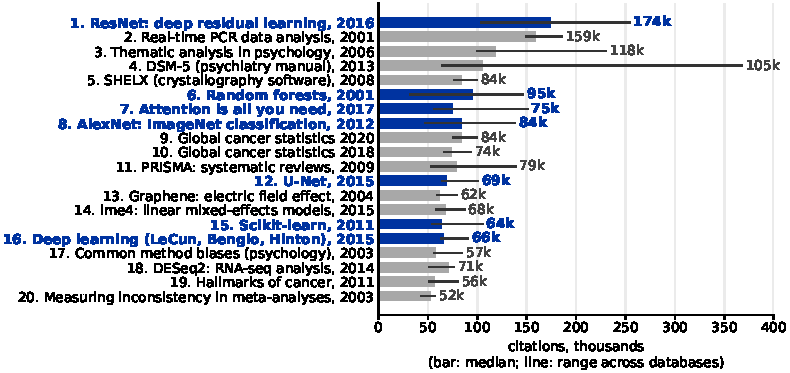
\includegraphics{most_cited_top20.pdf}\par}
  \vskip 3pt
  \footnotesize Machine learning in \textcolor{armblue}{\textbf{blue}}: 7 of 20. Five databases
  disagree by up to $5.7\times$ (Google Scholar is highest for 19 of 20), so Nature ranks by
  \emph{median rank}: the bars are not sorted. {\scriptsize\color{gray} Data: Nature 640,
  588-592 (2025), supplementary table, March 2025.}
\end{frame}

% 2026-10-01 (l17_todo #2): Welch Labs, "The most cited paper of the century is a brilliant hack",
% 2026-09-01, 35:18. Still = the video's cover image (i.ytimg.com maxresdefault) ->
% fig/borrowed/welchlabs_resnet_cover.jpg.
\mustwatch{welchlabs_resnet_cover.jpg}{Welch Labs, 2026}{https://www.youtube.com/watch?v=QgH9sr7G13Q}{The most cited paper of the century is a brilliant hack}{35 minutes on ResNet: why deep plain networks fail to train, and why one skip connection fixes it.}

% ================================================================
\section{After ImageNet, and in practice}

\begin{frame}[plain]
  \vfill
  \begin{center}
    {\Large\color{popblue}\textbf{After ImageNet}}\\[0.9em]
    \begin{minipage}{0.82\textwidth}\centering\small
      Sharper tricks, bigger searches, a saturated benchmark - and one import to get them all.
    \end{minipage}
  \end{center}
  \vfill
  \begin{center}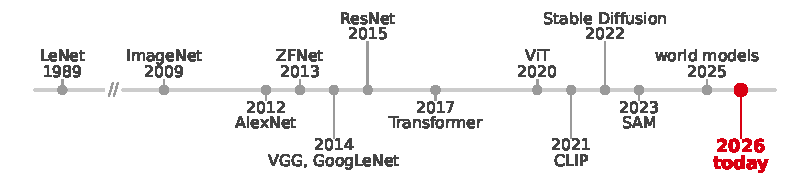
\includegraphics[width=5.4in]{ribbon_5.pdf}\end{center}
\end{frame}

\begin{frame}{Grouped convolution}
  \begin{columns}[T]
    \column{0.46\textwidth}
    \small
    Split the input channels into $g$ \textbf{groups}; each group gets its own filters,
    with no mixing across groups. Parameters and compute drop by a factor of $g$.
    \vskip 6pt
    \begin{itemize}\small
      \item You already saw it: \textbf{AlexNet}'s split made conv 2, 4, 5 grouped
        ($g=2$), one group per card (conv 3 crossed over).
      \item Push it to the extreme, \textbf{one group per channel} ($g=C$), and it is the
        \textbf{depthwise} convolution behind separable convs ([51]).
      \item \textbf{ResNeXt} (2017) made $g$ a design knob ("cardinality") - a third lever
        beside depth and width.
    \end{itemize}
    \column{0.54\textwidth}
    \begin{center}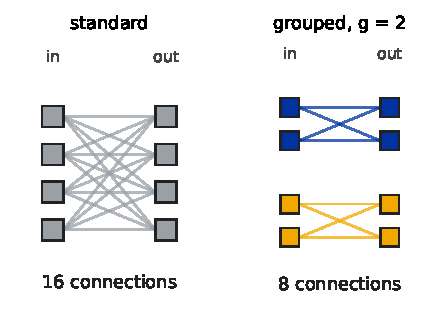
\includegraphics[width=0.92\linewidth]{grouped_conv_demo.pdf}\end{center}
    \vskip 2pt
    \fcolorbox{paramgreen}{paramgreen!8}{\parbox{0.95\linewidth}{\small
      $g{=}2$ (AlexNet) to $g{=}C$ (depthwise). \emph{Deformable} conv (Dai et al., 2017)
      even learns \emph{where} to sample.}}
  \end{columns}
\end{frame}

\begin{frame}{Scaling and searching}
  Where architecture design went next - one line each:
  \vskip 6pt
  \begin{itemize}
    \item \textbf{DenseNet}: like ResNet, but \emph{concatenate} the skip instead of
      adding it.
    \item \textbf{EfficientNet}: scale depth, width and resolution \emph{together}
      with one compound coefficient.
    \item \textbf{Neural architecture search}: architectures are now \emph{found} by
      search as much as designed by hand.
  \end{itemize}
  \vskip 8pt
  \fcolorbox{armblue}{armblue!8}{\parbox{0.97\linewidth}{\small
      None of these change the vocabulary you now have: conv blocks, skips,
      $1\times1$s, GAP. The d2l.ai chapter on modern CNNs covers each, for the
      curious.}}
\end{frame}

% 2026-10-01 (l17_todo #6). CoCa (Yu et al., arXiv 2205.01917): 91.0% top-1 fine-tuned, 86.3%
% zero-shot. Northcutt et al. 2021, "Pervasive label errors in test sets": 2,916 errors = 6% of
% the ImageNet validation set. Web-checked 2026-10-01.
\begin{frame}{ImageNet today}
  \begin{itemize}
    \item Top-5 error fell from $26\%$ (2011) to $3.6\%$ (2015). Since then papers report the
      stricter \textbf{top-1} accuracy: the best is about \textbf{91\%} (CoCa, 2022).
    \item \textbf{86\%} with \emph{no} ImageNet training at all: CoCa learned from billions of
      image-caption pairs and is only told the 1{,}000 class names (CLIP-style - epilogue).
    \item The test set is the limit now: about \textbf{6\% of ImageNet's validation labels are
      wrong} (Northcutt et al., 2021). Above 90\%, a "mistake" is often the label's.
  \end{itemize}
  \vskip 6pt
  \fcolorbox{armblue}{armblue!8}{\parbox{0.97\linewidth}{\small
    ImageNet is \textbf{solved enough} that it no longer ranks new models - they are compared on
    harder test sets (new photos, sketches, deliberately tricky images). It is still the
    default starting point for \textbf{transfer}: that is [50].}}
\end{frame}

\begin{frame}[fragile]{torchvision.models}
\begin{lstlisting}
import torch
from torchvision import models

net = models.resnet18(weights="IMAGENET1K_V1")  # pretrained
print(sum(p.numel() for p in net.parameters()))  # 11,689,512

net.fc = torch.nn.Linear(512, 3)  # new head: export/market/juice
\end{lstlisting}
  \vskip 4pt
  Load an architecture, inspect it, swap the head for \emph{your} classes - three
  lines each.
  \vskip 4pt
  \fcolorbox{paramgreen}{paramgreen!8}{\parbox{0.97\linewidth}{\small
      What "keep the body, replace the head" buys you - and when to also retrain the
      body - is the whole next lecture.}}
  \vskip 2pt
  \begin{center}
    \href{https://docs.pytorch.org/vision/stable/models.html}{\beamergotobutton{torchvision
    models docs}}
  \end{center}
\end{frame}

\begin{frame}{Which architecture, when}
  Back to the \textbf{pomegranate sorting line}:
  \vskip 8pt
  \begin{itemize}
    \item A Fashion-MNIST-sized toy problem (small grayscale crops, few classes)
      $\to$ the \textbf{small custom CNN from [48]}: 9k parameters, trains in
      minutes, easy to debug.
    \item The real sorting camera ($224\times224$ color photos, subtle grade
      differences) $\to$ start from a \textbf{pretrained ResNet-family model} and
      adapt it.
  \end{itemize}
  \vskip 10pt
  \fcolorbox{paramgreen}{paramgreen!8}{\parbox{0.97\linewidth}{
      Adapting a pretrained model to your data \emph{is} \textbf{transfer learning} -
      exactly where the next lecture picks up.}}
\end{frame}

% ================================================================
\section{Epilogue: the field in 2026}

\begin{frame}[plain]
  \vfill
  \begin{center}
    {\Large\color{popblue}\textbf{Where did the field go?}}\\[0.9em]
    \begin{minipage}{0.82\textwidth}\centering\small
      Fourteen years after AlexNet: what vision looks like in 2026.
    \end{minipage}
  \end{center}
  \vfill
  \begin{center}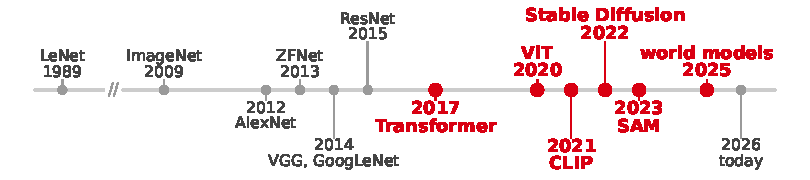
\includegraphics[width=5.4in]{ribbon_6.pdf}\end{center}
\end{frame}

\begin{frame}{Vision in 2026 (I): understanding}
  Two shifts since this lecture's timeline ended:
  \vskip 6pt
  \begin{enumerate}
    \item \textbf{Attention ate the frontier.} Vision Transformers (ViT) treat an
      image as a \emph{sequence of patches} - no convolution at all. ([51] closes
      this thought against CNN inductive bias.)
    \item \textbf{Image-text pretraining} (Contrastive Language-Image Pre-training,
      CLIP, 2021) fused vision with language: today's assistants (GPT, Gemini, Claude)
      are \textbf{vision-language models} (VLMs) - they \emph{see}: show them a photo,
      ask questions.
  \end{enumerate}
  \vskip 8pt
  \fcolorbox{armblue}{armblue!8}{\parbox{0.97\linewidth}{\small
      Classification stopped being a standalone task and became a \textbf{capability
      inside larger systems}.}}
  \vskip 4pt
  \begin{center}
    \href{https://claude.ai}{\beamergotobutton{try it: show a VLM a photo, ask it
    questions}}
  \end{center}
\end{frame}

% 2026-10-01: generator list refreshed (instructor-approved): GPT Image replaced DALL-E in ChatGPT
% (2025); Nano Banana = Google's Gemini image model (2025); Kling (Kuaishou), Seedance (ByteDance).
% SAM -> SAM 3 (Meta, 2025-11-19): concept prompts segment every instance, images and video.
\begin{frame}{Vision in 2026 (II): generation and segmentation}
  \textbf{Diffusion models flipped the task}: classification asks "what is this?" - diffusion
  answers "\emph{draw me one}".
  \vskip 6pt
  \begin{itemize}
    \item Images: Stable Diffusion, Flux, Google's Nano Banana, OpenAI's GPT Image. Video
      followed: Veo, Sora, Kling, Seedance.
    \item Intuition in one line: learn to \textbf{undo noise, step by step} - the mechanics
      belong to the diffusion chapter (L27-L31).
    \item Foundation models took the classic tasks too: \textbf{SAM 3} (Meta, 2025) - type a
      concept ("yellow school bus") and it segments \textbf{every} instance, in images and
      video, with no task-specific training.
  \end{itemize}
  \vskip 6pt
  \fcolorbox{paramgreen}{paramgreen!8}{\parbox{0.97\linewidth}{\small
      Generative vision gets its own treatment in the \textbf{diffusion chapter}
      (L27-L31) - here it is context, not curriculum.}}
  \vskip 4pt
  \begin{center}
    \href{https://aidemos.meta.com/segment-anything}{\beamergotobutton{SAM 3 demo: type a
    concept, get every mask}}
  \end{center}
\end{frame}

\begin{frame}{And yet: CNNs did not die}
  On phones, cars, cameras and sorting lines - including our \textbf{pomegranate
  belt} - CNNs and CNN hybrids remain the workhorse:
  \vskip 6pt
  \begin{itemize}
    \item \textbf{cheap and fast} at the edge, where there is no data center;
    \item the \textbf{right inductive bias} when data is limited ([48]'s whole
      argument);
    \item ResNets are still the \textbf{default baseline} in papers, a decade on;
    \item and given the same data and compute, convolution \textbf{keeps pace}:
      \textbf{ConvNeXt} (Liu et al., 2022) matched vision transformers with a pure-conv
      design, and DeepMind's NFNets matched them at web scale (Smith et al., 2023).
  \end{itemize}
  \vskip 8pt
  \fcolorbox{paramgreen}{paramgreen!8}{\parbox{0.97\linewidth}{
      You learned the layer that still does most of the world's looking.}}
\end{frame}

% ================================================================
\section*{Recap}

\begin{frame}{Recap}
  \begin{columns}[T]
    \column{0.55\textwidth}
    \begin{itemize}\small
      \item A shared \textbf{benchmark} (ImageNet: 1.2M photos, 1{,}000 classes) turned
        architecture design into measurable progress.
      \item \textbf{AlexNet} (2012) $=$ LeNet's blueprint $+$ [43]-[45]'s tricks at GPU
        scale; \textbf{ZFNet} (2013) looked inside and fixed it.
      \item \textbf{VGG} (2014): stacked $3\times3$ filters - same view, fewer weights.
        \textbf{GoogLeNet} (2014): parallel filter sizes, $1\times1$ bottlenecks, GAP -
        once the receptive field covers the object.
      \item \textbf{ResNet} (2015): deeper plain nets \emph{degrade} $\to$ residual learning
        ($=$ boosting in depth); skips also carry gradients.
      \item \textbf{Load pretrained models}; don't retype architectures. ImageNet is
        saturated, and CNNs still run the edge.
    \end{itemize}
    \column{0.43\textwidth}
    \fcolorbox{armblue}{armblue!8}{\parbox{0.95\linewidth}{\small
        \textbf{Practical - Gesture Snake.} Record your own thumb photos, then pit a
        small custom CNN against a pretrained ResNet-18 - and steer Snake with the
        winner.}}
    \vskip 6pt
    \fcolorbox{paramgreen}{paramgreen!8}{\parbox{0.95\linewidth}{\small
        \textbf{Next:} these models were trained on 1.2M images. You have 2{,}000. Transfer
        learning - stand on ImageNet's shoulders ([50]).}}
  \end{columns}
\end{frame}

\end{document}

% ================================================================
% Provenance:
%   Deck: L17 CNN Architectures (12_cnn). Built 2026-07-14 from
%   49_cnn_architectures_OUTLINE.md (approved, 3 interview rounds) +
%   CNN_CHAPTER_PLAN.md.
%
%   Sources consulted (REDERIVE, read-only): LMU I2DL cnn3/{modern-cnn-1,
%   modern-cnn-2}.tex, cnn1/architecture.tex. Credit line on title frame per
%   instructor decision (CC BY 4.0). All history facts from the outline's
%   verified-facts block, re-verified by web search 2026-07-14 (ILSVRC numbers,
%   GoogLeNet params "under 7M", Krizhevsky beat, SSI status, AMI Labs $1.03B,
%   link URLs).
%
%   Figures (py_src -> fig, ma venv): imagenet_error.py (imagenet_error.pdf +
%   imagenet_anim_0..6.pdf flip-book - cold open, winner names revealed with bars);
%   pretrained_filters.py (resnet18 conv1 8x8 RGB grid, one-time ~45MB weight
%   download - sanctioned, kept after the no-dataset-downloads scope change);
%   receptive_field.py (nested-fields grid + 27C^2-vs-49C^2 bars);
%   timeline_ribbon.py (ribbon_1..6.pdf, one per section transition, "you are
%   here" in red). cifar_grid.py was DROPPED (instructor scope change 2026-07-14:
%   no dataset downloads) - the recap's CIFAR-10 grid is WEB-IMG instead
%   (cifar10_grid.png, the PyTorch-tutorial class grid).
%
%   WEB-IMG (fig/borrowed/, no credit lines per standing policy): lenet_arch.pdf,
%   inception_block.pdf, residual_block.pdf, googlenet_full.pdf (all d2l.ai SVGs
%   -> cairosvg PDF; googlenet uses the 90-degree horizontal variant);
%   alexnet_twogpu.png (AlexNet paper Fig 2 crop), he_degradation.png (He et al.
%   2015 Fig 1 crop), imagenet_samples.png (AlexNet paper Fig 4 left panel crop -
%   real ILSVRC test photos + top-5 bars, doubles as the top-5-error illustration);
%   cifar10_grid.png (PyTorch-tutorial CIFAR-10 class grid, recap frame).
%   degradation.py superseded per round-3 decision (iconic originals).
%
%   Key decisions (details in 49_DECISIONS.md): winner names moved into the
%   chart's tick labels so anim frames don't spoil the reveal; ILSVRC 2012 error
%   16.4 (winning entry, no outside data; 15.3 was the extra-data variant);
%   GoogLeNet params stated as "under 7M" (sources vary 5-6.8M); receptive-field
%   pointer corrected L18 -> L19 (4-deck split moved dilated convs); VLM link =
%   claude.ai; SAM link = sam2.metademolab.com (segment-anything.com DNS failed at
%   build time); two link buttons on the LeNet frame (outline names both).
%
%   Facts kept soft per outline: "an estimated 10-20% of US checks"; Krizhevsky
%   "quietly stepped away from the field"; no portraits anywhere (locked).
%
%   2026-07-21 addition (instructor request, after a coverage check vs standard
%   convolution-type taxonomies): new "Grouped convolution" frame before "Scaling and
%   searching" - names AlexNet's two-GPU split as grouped conv (g=2), bridges to depthwise
%   (g=C, L19) and ResNeXt cardinality. Figure grouped_conv_demo.pdf (py_src -> fig, ma venv:
%   standard 16 vs grouped-g2 8 channel connections, asserted). Same frame carries a one-line
%   deformable-convolution name-drop (Dai et al. 2017). Prompted by the 3Blue1Brown
%   convolution mining (see _reference_3b1b_convolution/).
%
%   2026-09-22 pre-delivery pass (instructor away - autonomous): retired L14/L15 callbacks
%   repointed to the delivered decks, each checked against the deck + its LMU pages:
%   GPU argument -> [42] (LMU 05_hardware-and-software), ReLU -> [45], dropout and
%   augmentation -> [43], vanishing gradients -> [42] + [45], BatchNorm formula -> [44].
%   AlexNet frame gained the paper's own ReLU number (4-layer CNN reaches 25% training error
%   on CIFAR-10 6x faster than tanh - Krizhevsky et al. 2012, Fig. 1). "CNNs did not die"
%   gained ConvNeXt (Liu et al., CVPR 2022) and NFNets at JFT-4B scale (Smith, Brock,
%   Berrada & De, arXiv 2310.16764, 2023). LeCun frame: AMI Labs' $1.03B round confirmed
%   (TechCrunch, 2026-03-09). SSI line dated "through August 2026" (no model/paper/product as
%   of 2026-08-24; an August release was only a podcast rumour, and a 2026-08-25 "debuting
%   this week" report was never confirmed by SSI). RE-CHECK BEFORE DELIVERY. All web-verified 2026-09-22.
%
%   Same day, after a Sonnet student review of the rendered deck: "Why skips also fix
%   gradients" gained a scalar worked example (0.5^20 ~ 1e-6 plain vs 0.9^20 ~ 0.12 ..
%   1.1^20 ~ 6.7 residual) and an honest footnote - He et al. 2015 Sec. 4.1 state the
%   degradation is "unlikely to be caused by vanishing gradients" because their plain nets
%   used BN and "the backward propagated gradients exhibit healthy norms" (quoted from the
%   arXiv PDF), so the deck no longer implies degradation == vanishing gradients. The
%   degradation box now says WHY identity is hard for a plain stack. Grouped-conv bullet
%   made exact from the AlexNet paper Sec. 3.5: conv 2, 4, 5 connect only to same-GPU maps;
%   conv 3 and the FC layers connect across (the old "the split WAS a grouped conv" was
%   true for 3 of 5 conv layers). GAP frame answers "why average, not max".
%
%   2026-09-30 error fixes (folder now ml/12_cnn): receptive-field box said dilated convs
%   were "coming in L19" - L16 teaches them since 2026-07-21, now "L16's ..., back in L19";
%   "thirteen years on" -> "fourteen" (2012 -> 2026 delivery).
%
%   2026-10-01 round 2 (instructor's l17_todo.md, 10 items; restructured by a scratchpad script
%   that lifted every kept frame verbatim by title):
%   - ORDER is now chronological: cold open (ImageNet photos, then the chart) -> benchmark ->
%     the breakout (LeNet, AlexNet, ZFNet) -> 2014 (receptive field, VGG, Inception/GoogLeNet,
%     dense head, GAP) -> 2015 ResNet -> after ImageNet + practice -> epilogue. Ribbons redrawn
%     to match (timeline_ribbon.py, broken axis, slide size).
%   - NEW: "ImageNet: 14 million photos..." (Deng et al. 2009 Fig. 1), "AlexNet: the rest of the
%     story" (margin, cuda-convnet, $44M auction, 2025 code release, Nature rank 8), "ZFNet (2013)"
%     (Zeiler & Fergus Fig. 2 + Sec. 4.1 facts), "VGG (2014): small filters, stacked" (cost table +
%     vgg_cost.pdf) and "VGG-16, layer by layer" (vgg_layout.py, totals checked vs torchvision),
%     GoogLeNet facts (names, CPU-only, from the paper), "What GoogLeNet sees: an activation atlas"
%     (Distill 2019), "ResNet (2015): the numbers" (Nature's most-cited list), "ImageNet today"
%     (CoCa 91.0% / 86.3% zero-shot, 6% label errors), two Welch Labs \mustwatch frames.
%   - Receptive field moved BEFORE VGG (VGG's argument needs it); VGG now argues 3x3x3 vs 7x7
%     with the receptive-field frame's own numbers.
%   - ILSVRC frame caption explains the red bar (AlexNet paper, Fig. 4 caption); AlexNet frame says
%     the diagram is cut off in the published paper itself (checked in the NeurIPS PDF).
%   - REMOVED: "The pioneers today" and "One paper, three fates" (instructor), and with them the
%     LeNet frame's "LeCun returns at the end" box. The Fei-Fei Li / World Labs line went too.
%   - Vision 2026 (II): generator list refreshed; SAM -> SAM 3 with its demo link.
%   - Figures redrawn at slide size: imagenet_anim_*, ribbons, receptive_field (+ vgg_cost split
%     out), grouped_conv_demo, pretrained_filters (title moved to the slide).
%
%   2026-10-01 pass (instructor request "improve slides"; web-checked 2026-10-01):
%   - NEW frame "When averaging away where hurts" after the GAP frame (instructor-approved):
%     the Gesture Snake known-answer test, flatten 77% / GAP 25% / ResNet-18 probe 99.6%
%     (DECISIONS #57), explained by receptive field (44 px of 128 for the small net).
%   - SSI: "through August 2026 ... a first model is rumoured" -> "through September 2026 ...
%     a rumoured August launch did not happen" (no model/paper/product as of 2026-09-25).
%     RE-CHECK BEFORE DELIVERY.
%   - LeCun: "~12 years as Meta's chief AI scientist" was wrong - he founded FAIR (Dec 2013)
%     and was chief AI scientist from 2018; now "~12 years at Meta - founding its AI research
%     lab, then as chief AI scientist". AMI and JEPA spelled out.
%   - Fei-Fei Li added to "The pioneers today": World Labs (3D world models), AMD agreed to
%     buy it for $8.2B on 2026-09-28 (all-stock, close expected end of 2026), Li to become AMD
%     chief scientist (CNBC, Bloomberg, Fortune, Tom's Hardware). Simonyan re-checked: still
%     Chief Scientist, Microsoft AI.
%   - Acronyms spelled out: ILSVRC, GAP, CLIP, VLM; recap BN -> BatchNorm.
%   - Recap: CIFAR-10 grid + "HW2's arena" caption (HW2 never built) replaced by a Gesture
%     Snake box (DECISIONS #58); GAP bullet gained the receptive-field caveat.
%   - 2026-10-01 late: the Gesture Snake notebook dropped its flatten-vs-GAP part (DECISIONS
%     #57 revisit: on real recordings both small heads fail). The "When averaging away where
%     hurts" numbers are still the measured synthetic ones; only its caption changed from
%     "the practical's known-answer test" to "measured while building the practical".
%   - 2026-10-02 (instructor): "One chart, one question" shows one note per winner on its own
%     click (2010 NEC-UIUC and 2011 XRCE too; AlexNet's note no longer stays up for 2013-2014).
%     Methods per Russakovsky et al. IJCV 2015 (2010: SIFT + LBP, non-linear coding, SVMs; 2011:
%     compressed Fisher vectors, linear SVMs). NEW frame "The top 20, with their citation counts"
%     (most_cited.py) built from Nature's own supplementary xlsx, kept in ml/12_cnn/data/; a
%     secondary web copy of the table had two duplicated numbers and a wrong year, so it was
%     not used. Caption facts computed from the sheet: Google Scholar highest for 19 of 20, max
%     spread 5.7x (DSM-5).
%
%   Forward pointer: L18 Transfer Learning - freeze vs fine-tune, the BatchNorm
%   gotcha, Grad-CAM/Clever Hans, labeling economics. L17's pretrained_filters
%   frame is the "why transfer works" anchor L18 calls back to.
%
%   2026-10-15: renumbered to the playlist after delivery (instructor: no practical between
%   [48] and transfer learning): [50] -> [49], [51] -> [50], [52] -> [51], the practical
%   [53] -> [52]; deck files renamed to match. Slide text uses the new labels; labels written in
%   this block before this date keep the old ones.
